\section{Results}
    In this section, we will present the results of all three experiments. In the heatmaps, the by red enclosed cells indicates the environments from the testing set used for extrapolation testing, while the non-red-enclosed cells represent the environments from the training set used for interpolation testing. Lastly, we will present the results on the different types of morphologies evolved in our experiments. Visualizations of these evolved MC-pairs from our different experiments can be viewed online\footnote{See the visual demonstration of the behaviors of the MC-pairs at: \url{https://www.youtube.com/watch?v=CWxKFhSb94I}}.
    \subsection{Experiment 1: One generalist}
        \begin{figure*}[!ht]
            \centering
            \begin{subfigure}{\textwidth}
                \centering
                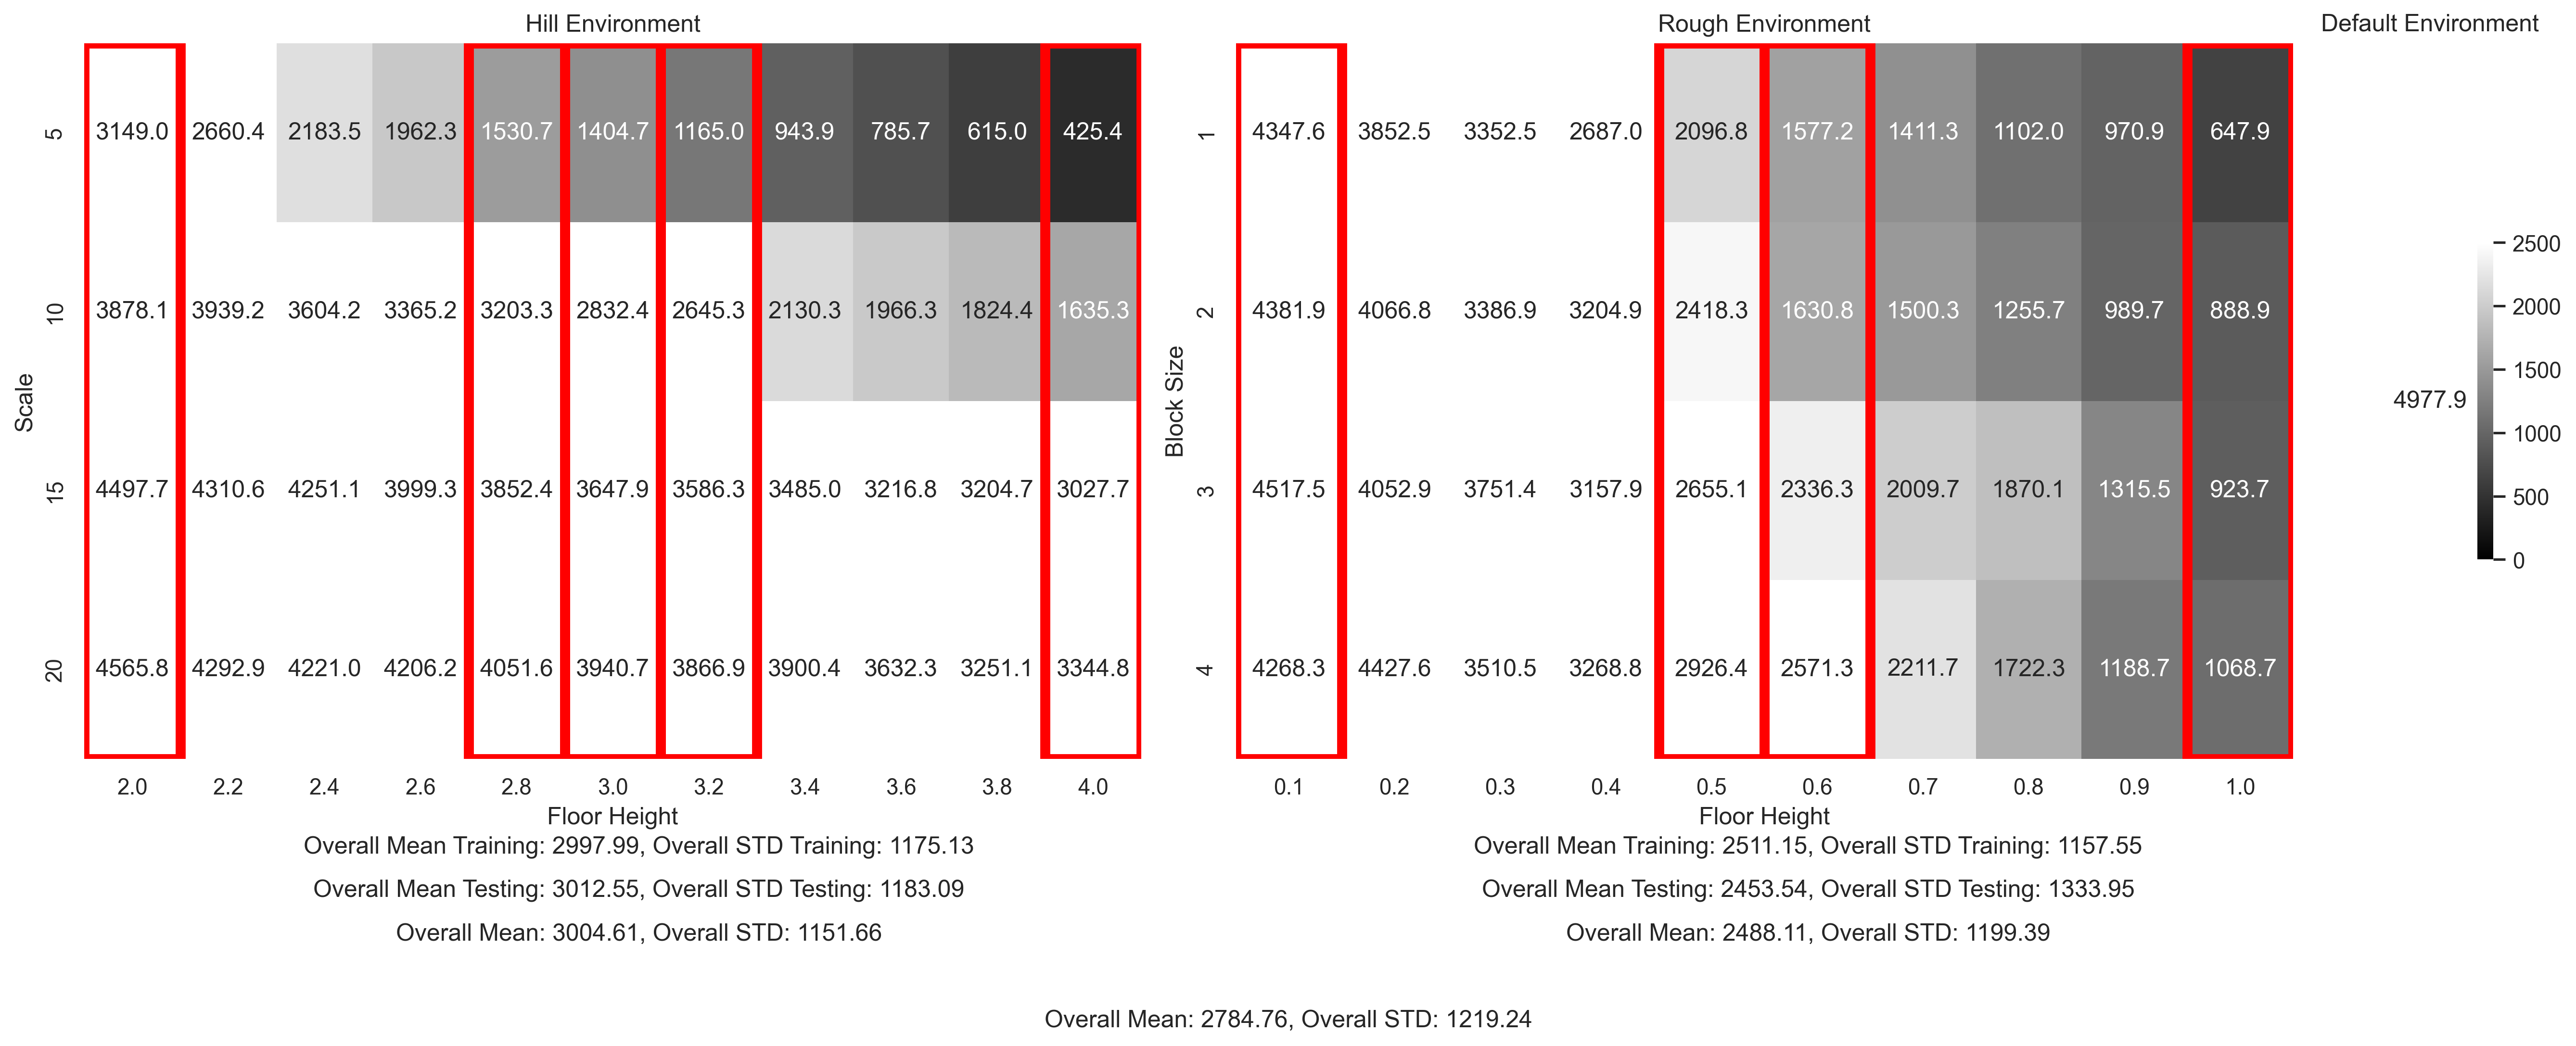
\includegraphics[width=\linewidth]{./resources/generalist_4_2784/fitness_heatmap.png}
                \caption{Fitness heatmap from one generalist MC-pair evolved over 5000 generations with partitions disabled}
                \label{fig:fit_heat_generalist}
            \end{subfigure}

            \begin{subfigure}{\textwidth}
                \centering
                \begin{minipage}{0.19\textwidth}
                    \centering
                    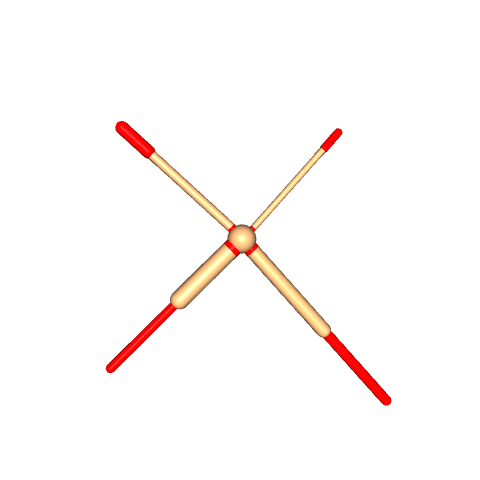
\includegraphics[width=\linewidth]{resources/generalist_2_2350/ant.png}
                    \textbf{2350}
                \end{minipage}
                \hfill
                \begin{minipage}{0.19\textwidth}
                    \centering
                    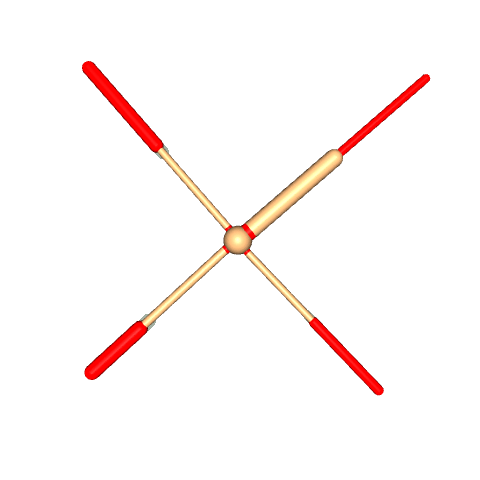
\includegraphics[width=\linewidth]{resources/generalist_3_2412/ant.png}
                    \textbf{2412}
                \end{minipage}
                \hfill
                \begin{minipage}{0.19\textwidth}
                    \centering
                    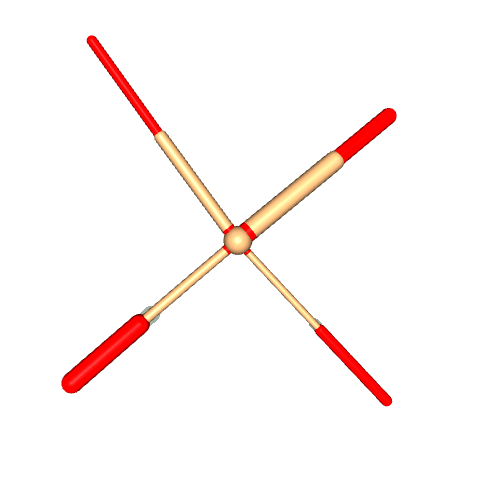
\includegraphics[width=\linewidth]{resources/generalist_4_2784/ant.png}
                    \textbf{2784}
                \end{minipage}
                \hfill
                \begin{minipage}{0.19\textwidth}
                    \centering
                    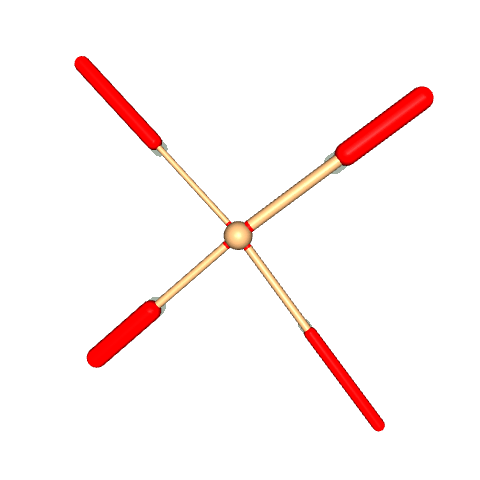
\includegraphics[width=\linewidth]{resources/generalist_1_2966/ant.png}
                    \textbf{2966}
                \end{minipage}
                \hfill
                \begin{minipage}{0.19\textwidth}
                    \centering
                    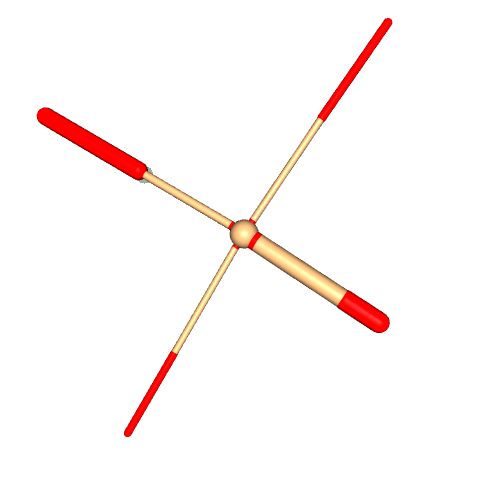
\includegraphics[width=\linewidth]{resources/generalist_5_3126/ant.png}
                    \textbf{3126}
                \end{minipage}

                \caption{Morphology evolved for one generalist MC-pair from different evolutionary runs ordered by generalist score, which is shown below the image.}
                \label{fig:gen_ant_images}
            \end{subfigure}
            
            \begin{subfigure}{\textwidth}
                \centering
                \begin{minipage}{0.32\textwidth}
                    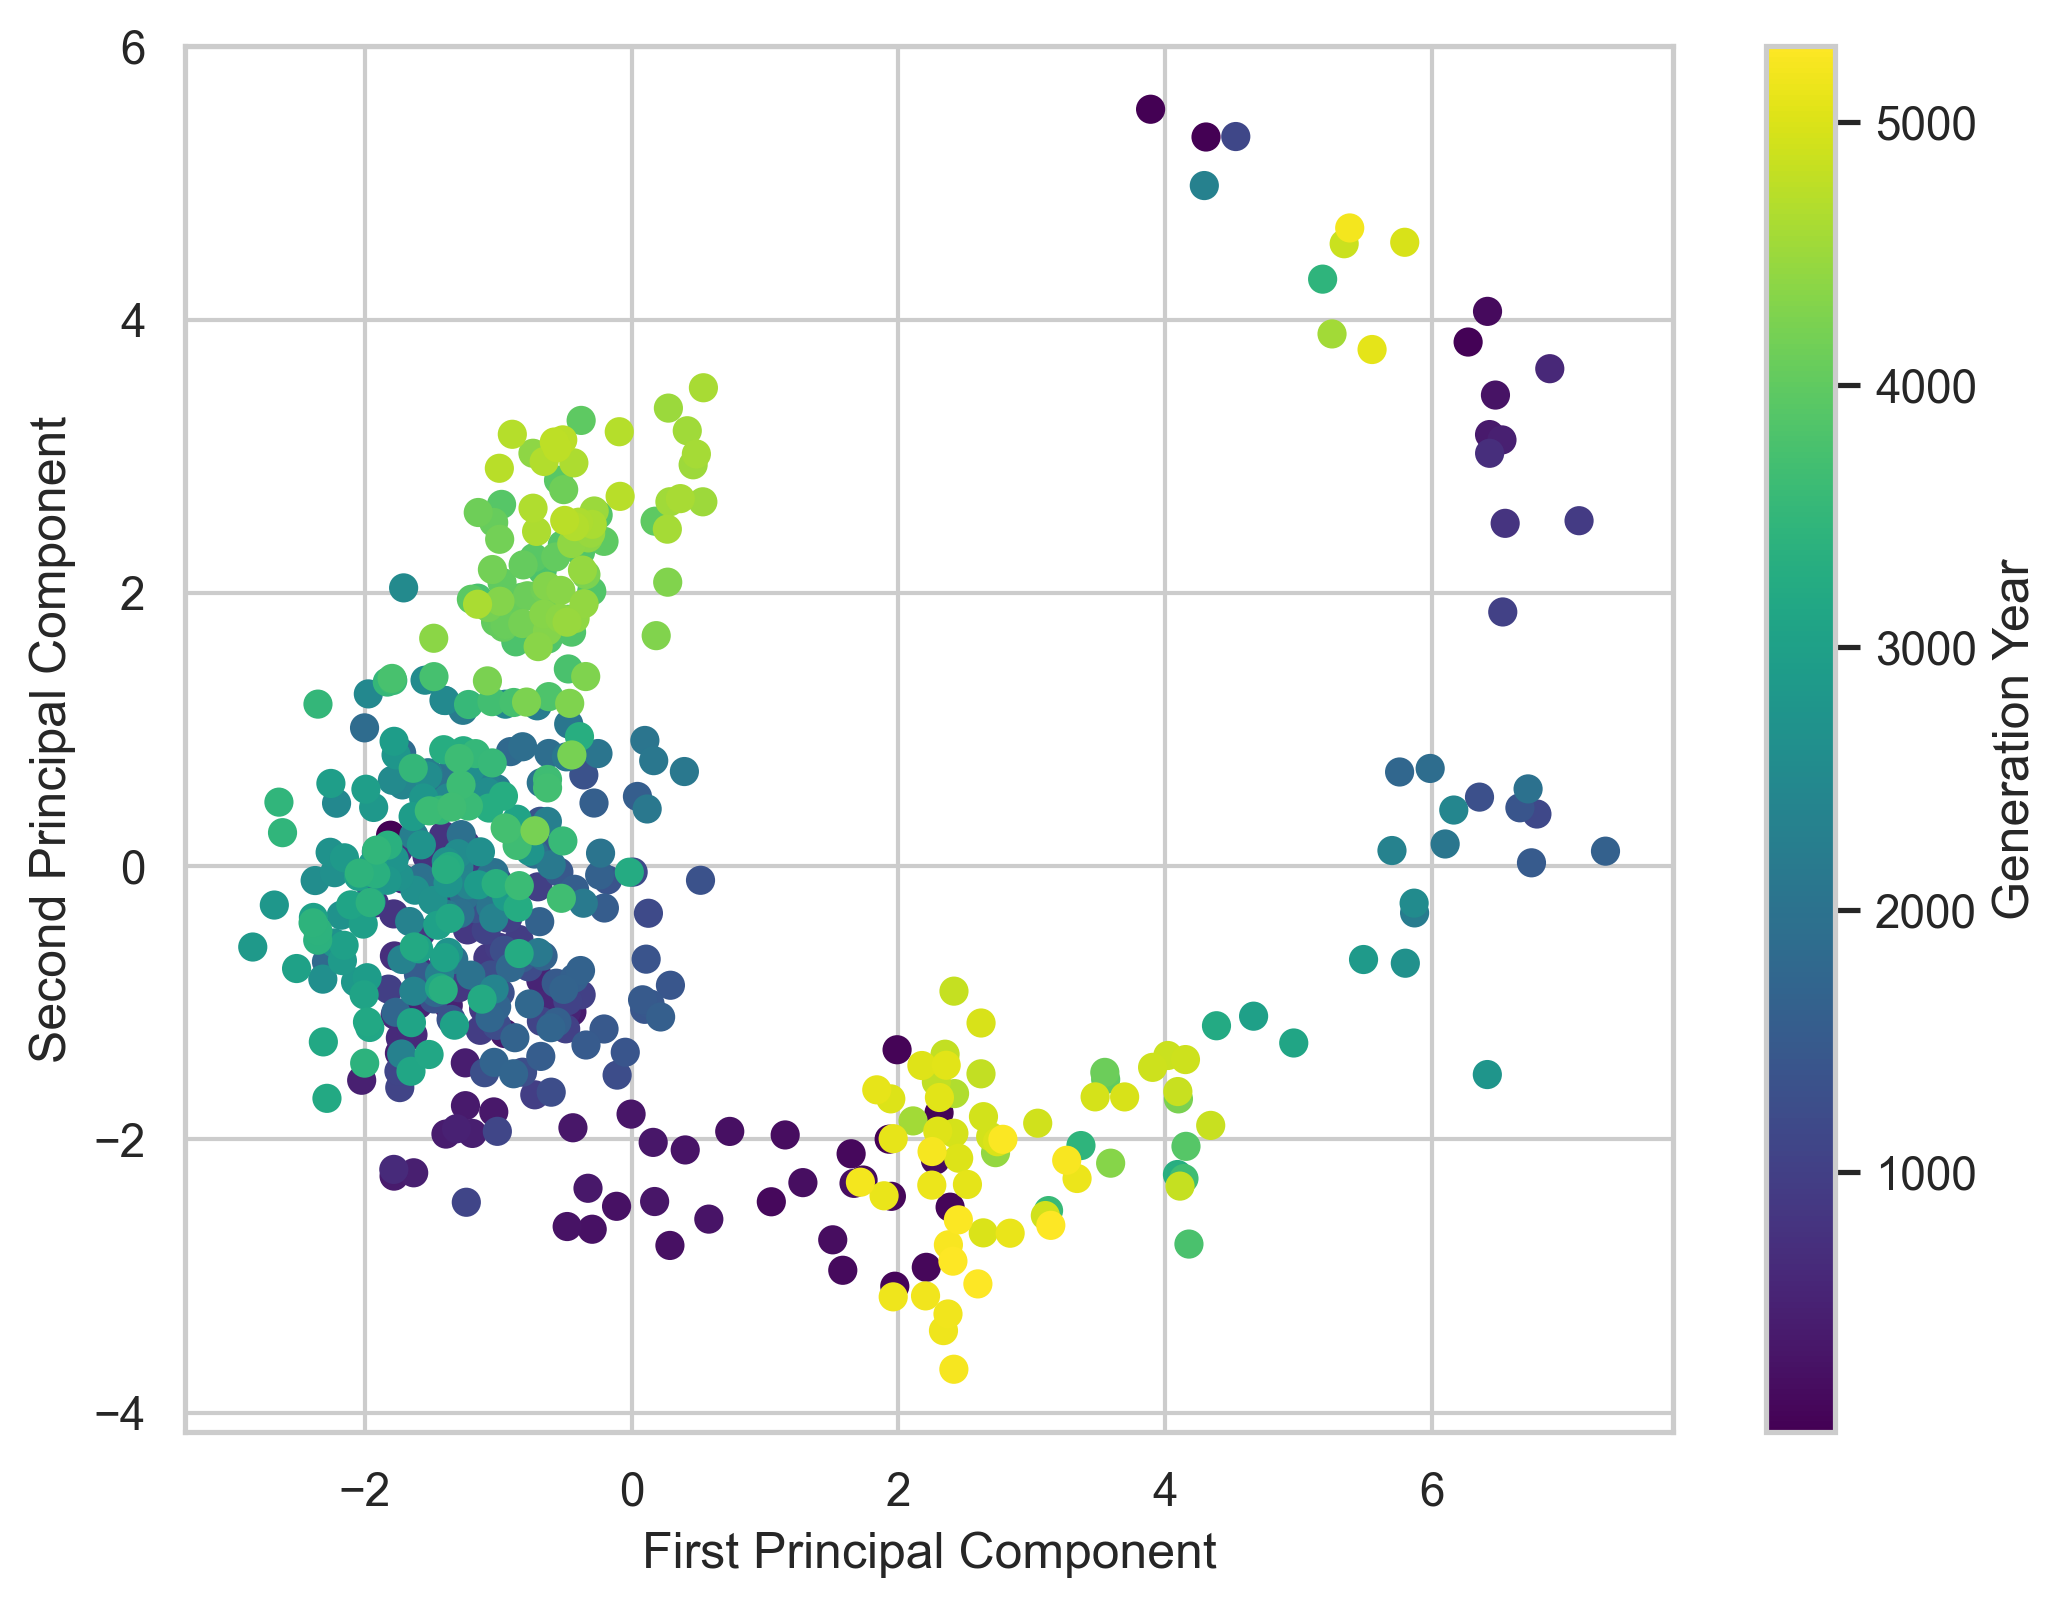
\includegraphics[width=\textwidth]{./resources/generalist_3_2412/pca_scatterplot.png}
                    \centering
                    \textbf{2412}
                \end{minipage}
                \hfill
                \begin{minipage}{0.32\textwidth}
                    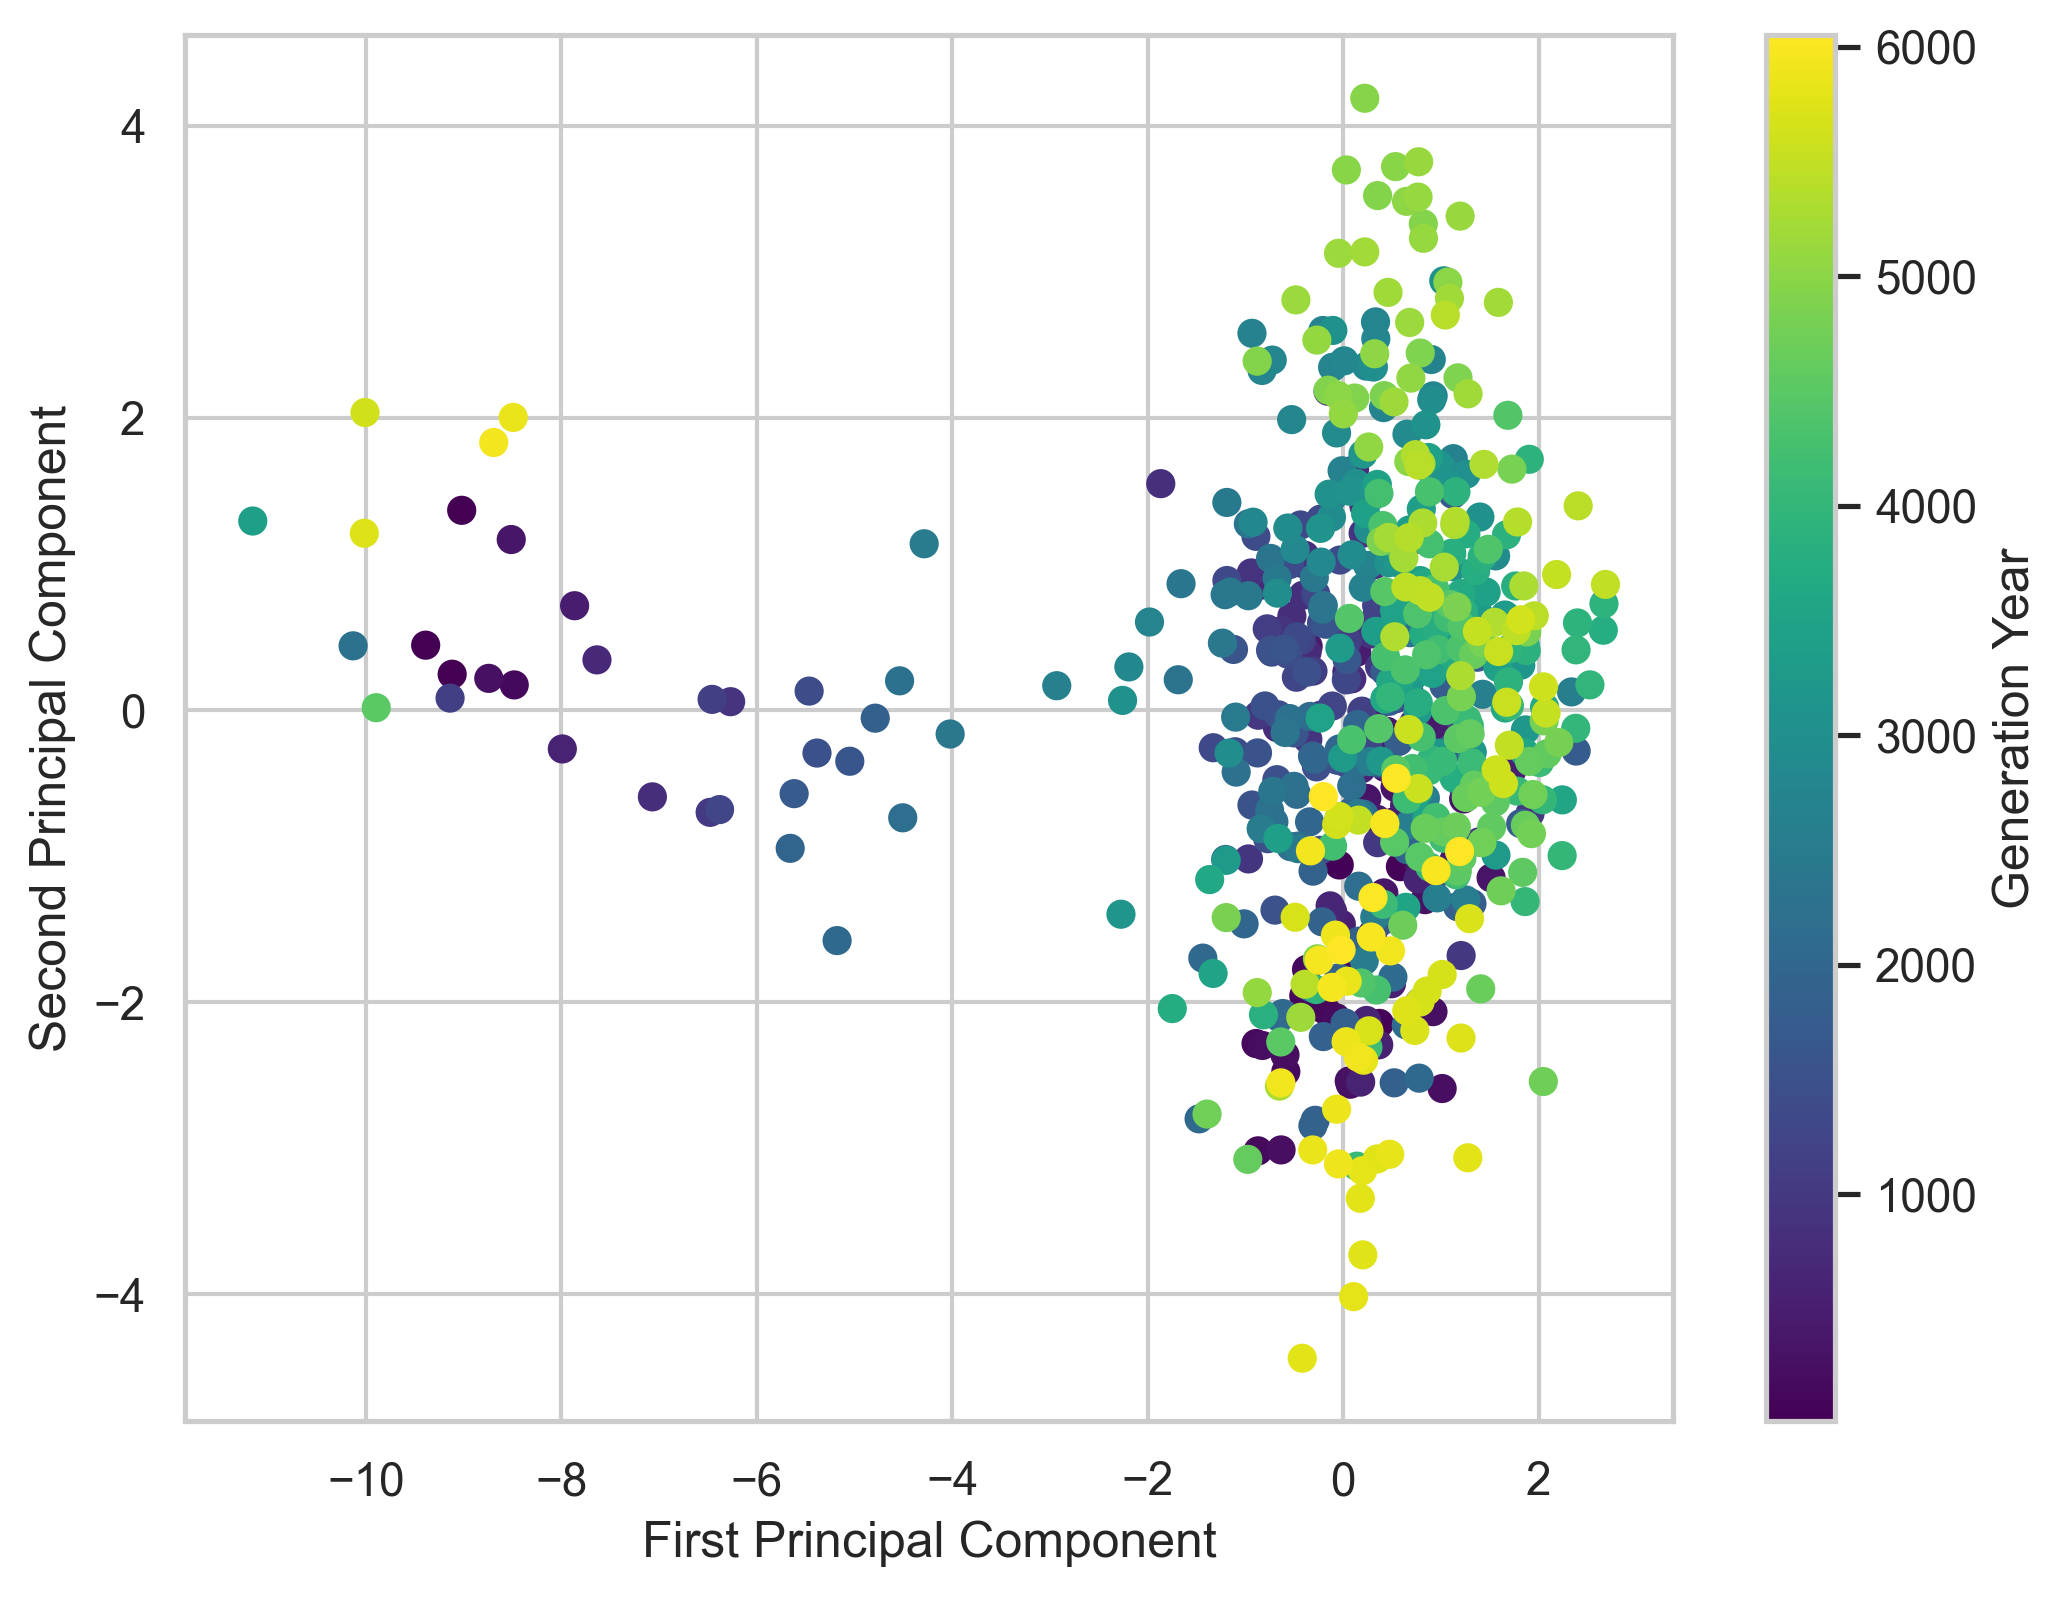
\includegraphics[width=\textwidth]{./resources/generalist_4_2784/pca_scatterplot.png}
                    \centering
                    \textbf{2784}
                \end{minipage}
                \hfill
                \begin{minipage}{0.32\textwidth}
                    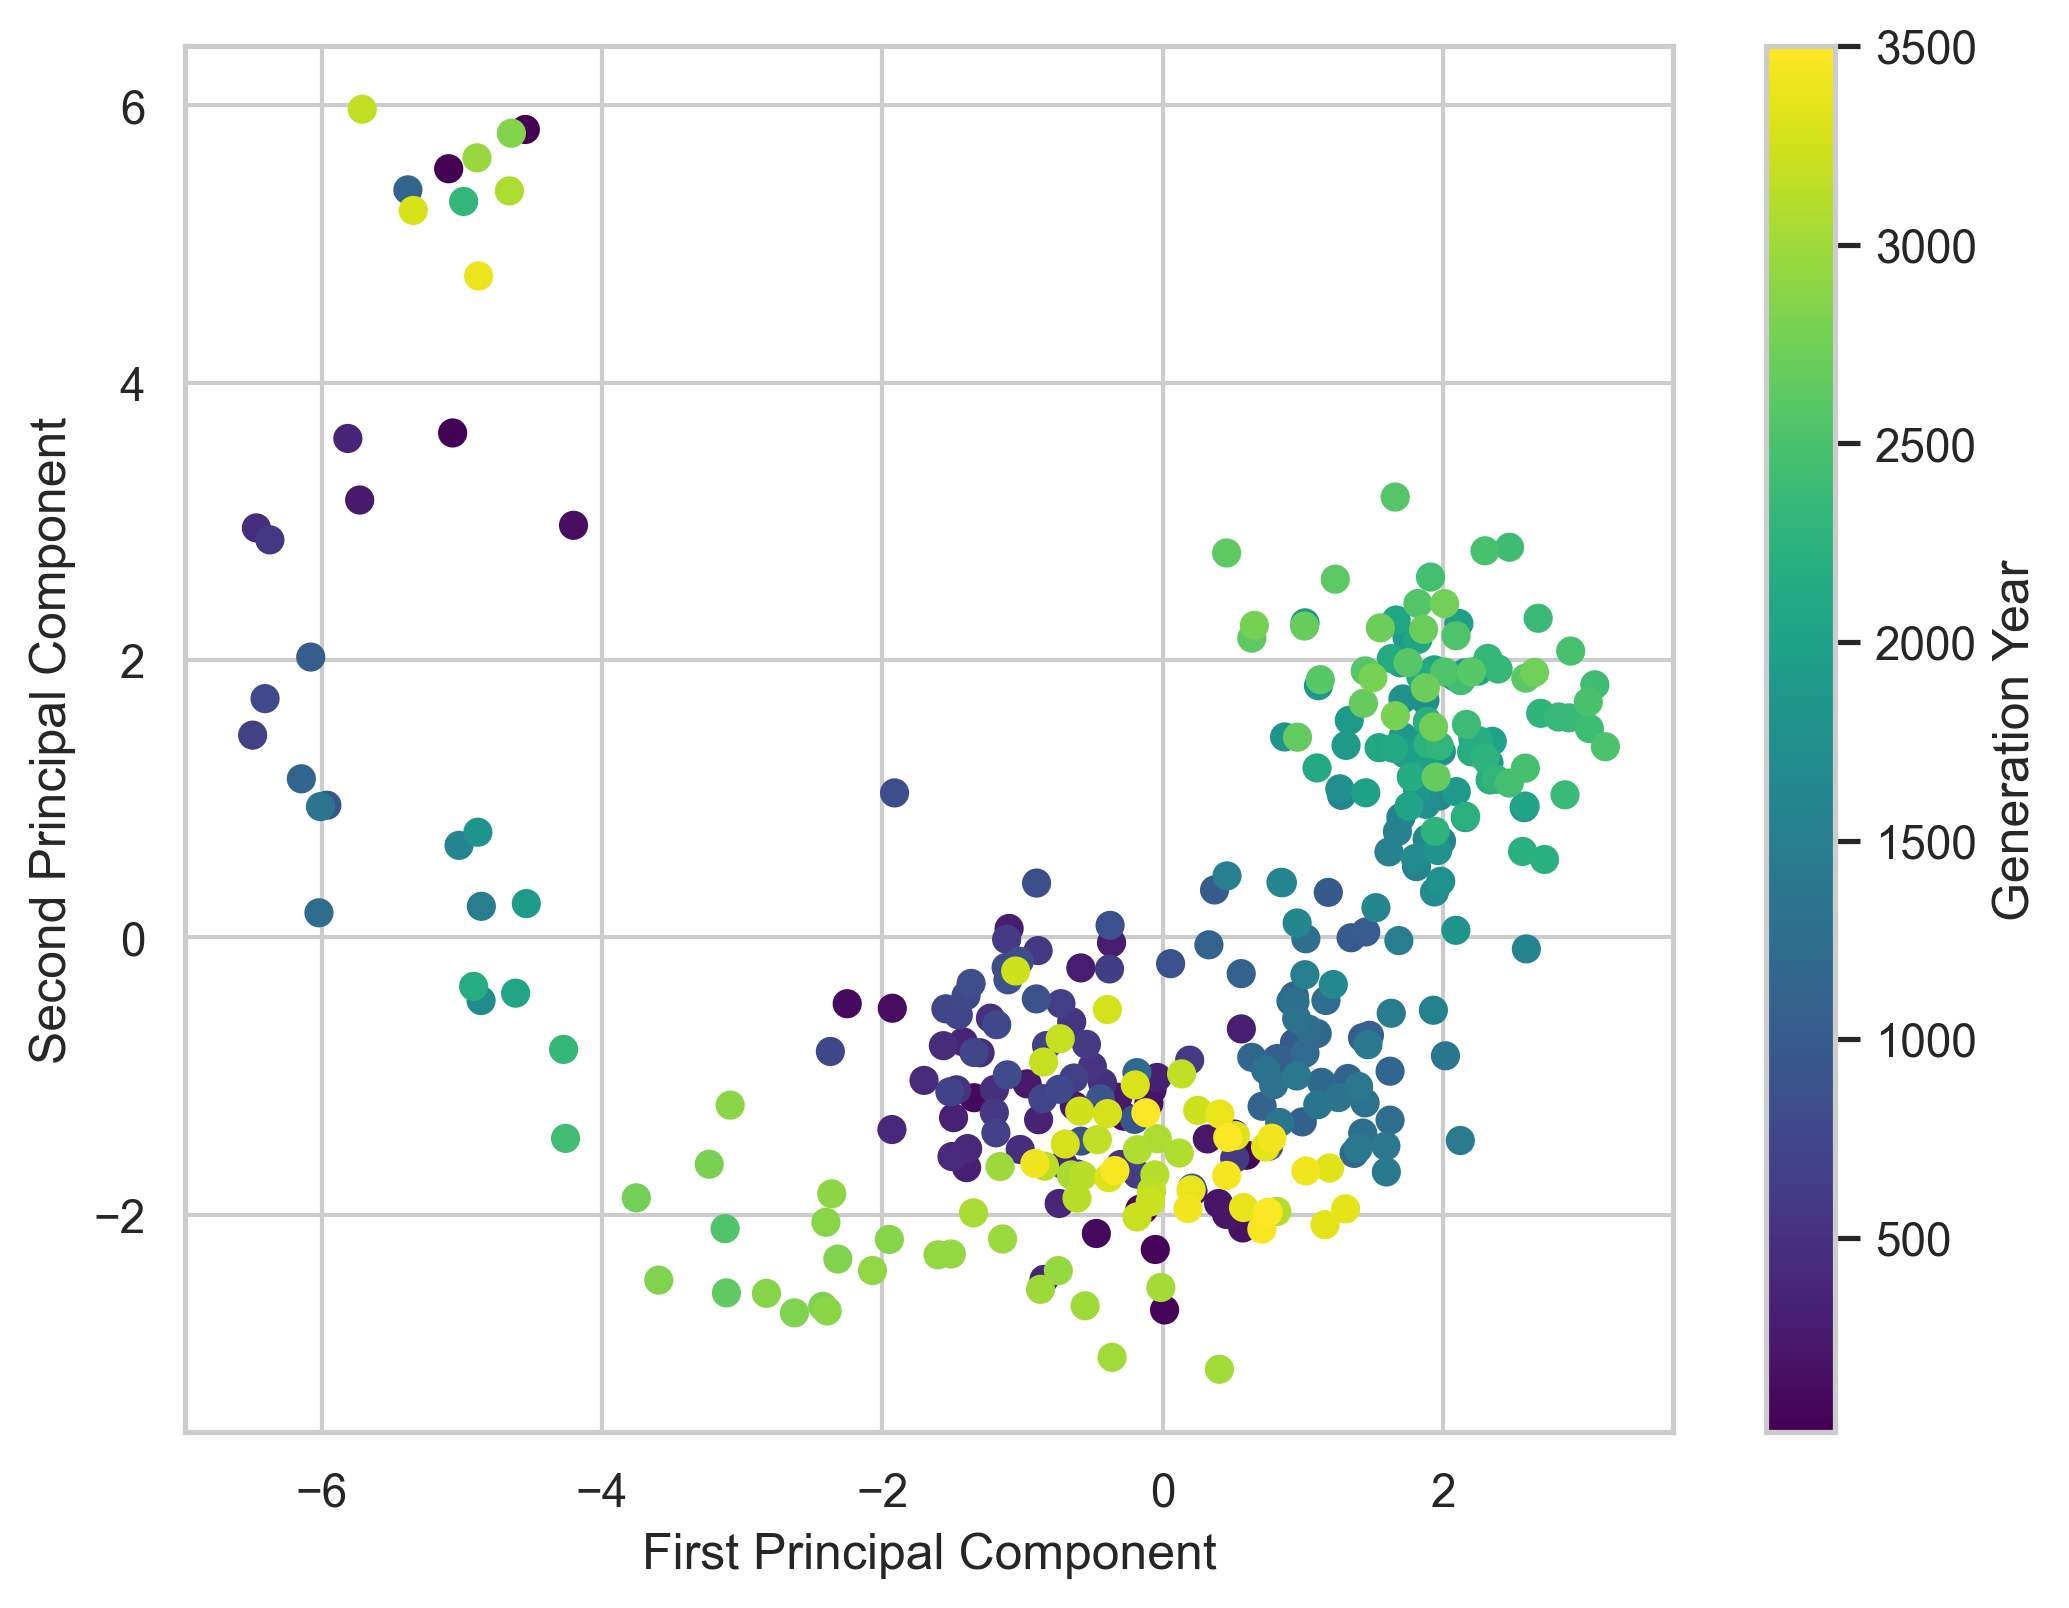
\includegraphics[width=\textwidth]{./resources/generalist_5_3126/pca_scatterplot.png}
                    \centering
                    \textbf{3126}
                \end{minipage}
                \hfill
                \caption{PCA scatterplots where the morphological parameters are reduced to 2 principal components with generalist scores shown below.}
                \label{fig:pca_generalist}
            \end{subfigure}

            \caption{Experiment 1 - Results of the first experiment where we evolve one generalist MC-pairs to handle a wide range of diverse environments.}
            \label{fig:experiment1}
        \end{figure*}

        Figure~\ref{fig:fit_heat_generalist} shows the obtained fitness scores for each environment, represented in a heatmap for experiment 1. For the hill environment, the heatmap shows high performance in the environments at the lower left and relatively lower performance when nearing the the upper right. This may indicate inherint complexity in certain environments compared to others. The fitness scores and their standard deviations on the training and testing sets are similar. The training set has a mean fitness score of 2997.99 with a standard deviation of 1175.13, and the testing set has a mean fitness score of 3012.55 with a standard deviation of 1183.09. 
        
        For rough terrain environment, the heatmap also shows high performance in the environments at the lower left and relatively lower performance when nearing the upper right, but also more at the lower right part. The fitness scores and their standard deviations on the training and testing sets are also similar. The training set has a mean fitness score of 2511.15 with a standard deviation of 1157.55, and the testing set has a mean fitness score of 2453.54 with a standard deviation of 1333.95.
        
        A significant factor that determined the fitness score and the strategy utilized to achieve this score was the evolved morphology. In experiment 1, we conducted a total of five evolutionary runs, and the resulting MC-pairs are visible in Figure~\ref{fig:gen_ant_images}. These images are ordered by the generalist score obtained, which is shown below each image. The ants with generalist scores 2412, 2784, and 3126 have similar morphological structures and employed very similar strategies to move forward, using its two side legs accellerate itself forward. In contrast, the ant with generalist score 2966 uses a more conventional strategy, resembling more of how an actual ant would move.

        In order to to visualize the search for morphology, we employed principal component analysis (PCA) to reduce the dimensionality of the morphological parameters from 16 to 2 principal components, enabling us to plot them on a 2D graph. Figure~\ref{fig:pca_generalist} shows a scatterplot where each point represents a different morphology, with the color indicating the generation where that morphology was encountered and validated as the generalist. Across all three plots, there is no clear gradient towards a specific morphological structure, and morphological changes can even still occur very late in the evolutionary run. The scatterplots for generalist scores 2412 and 3126 shows that the search is happening within a circular-like space in the morphology space, whereas for generalist score 2784, the search begins with a morphology and tended to stick with its initialy generated morphology. 

    \subsection{Experiment 2: Partitioned generalist}
        \begin{figure*}[!htp]
            \centering
            \begin{subfigure}{\textwidth}
                \centering
                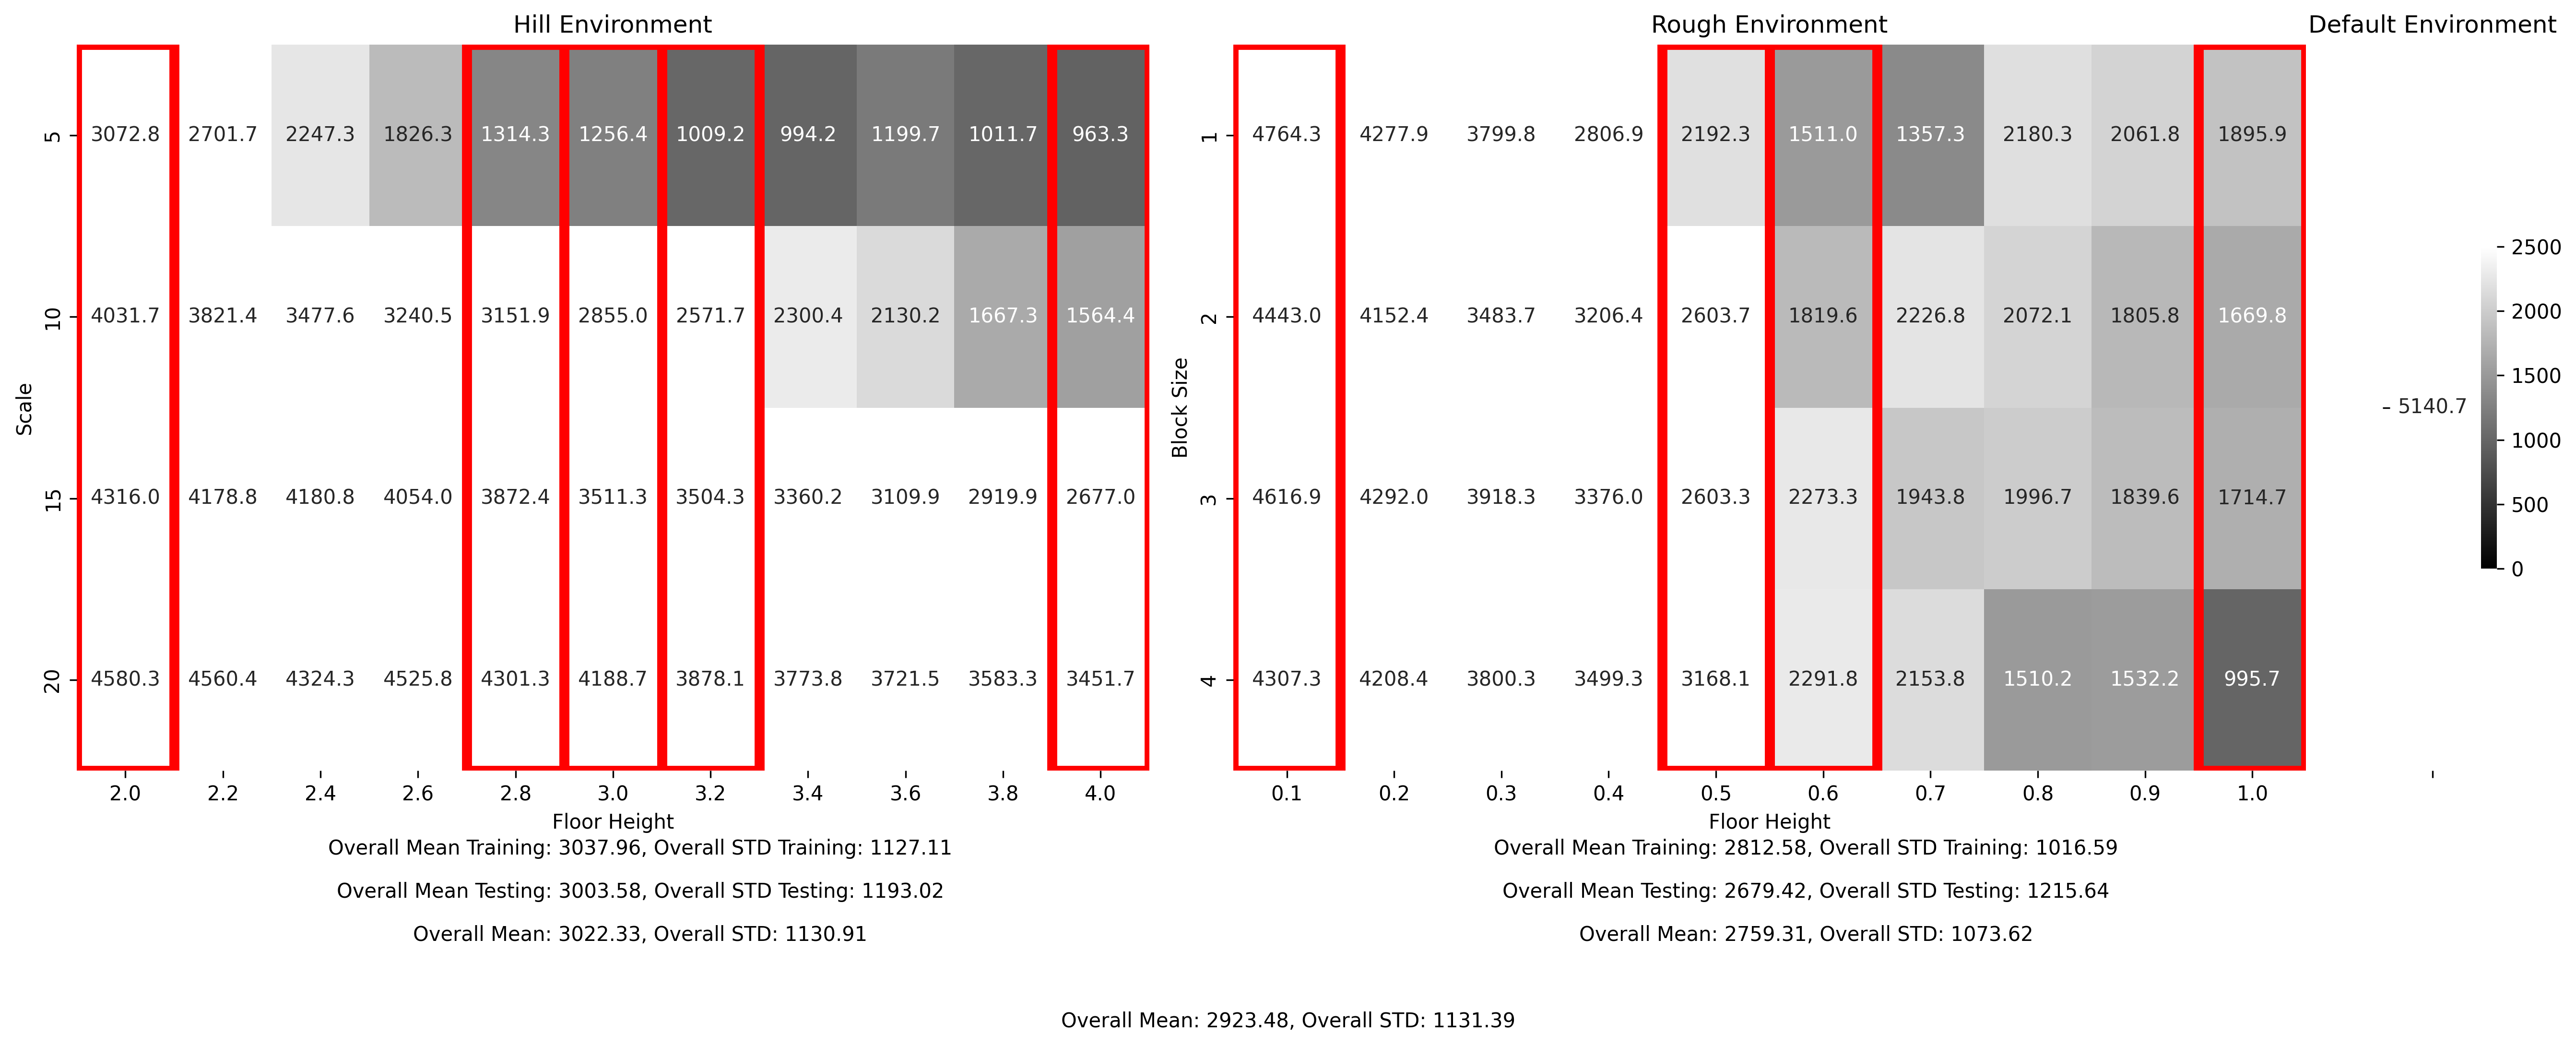
\includegraphics[width=\linewidth]{./resources/partition_5_2906_3/fitness_heatmap.png}
                \caption{Fitness heatmap of a set of generalist MC-pair}
                \label{fig:fit_heat_partitioned}
            \end{subfigure}

            \begin{subfigure}{\textwidth}
                \centering
                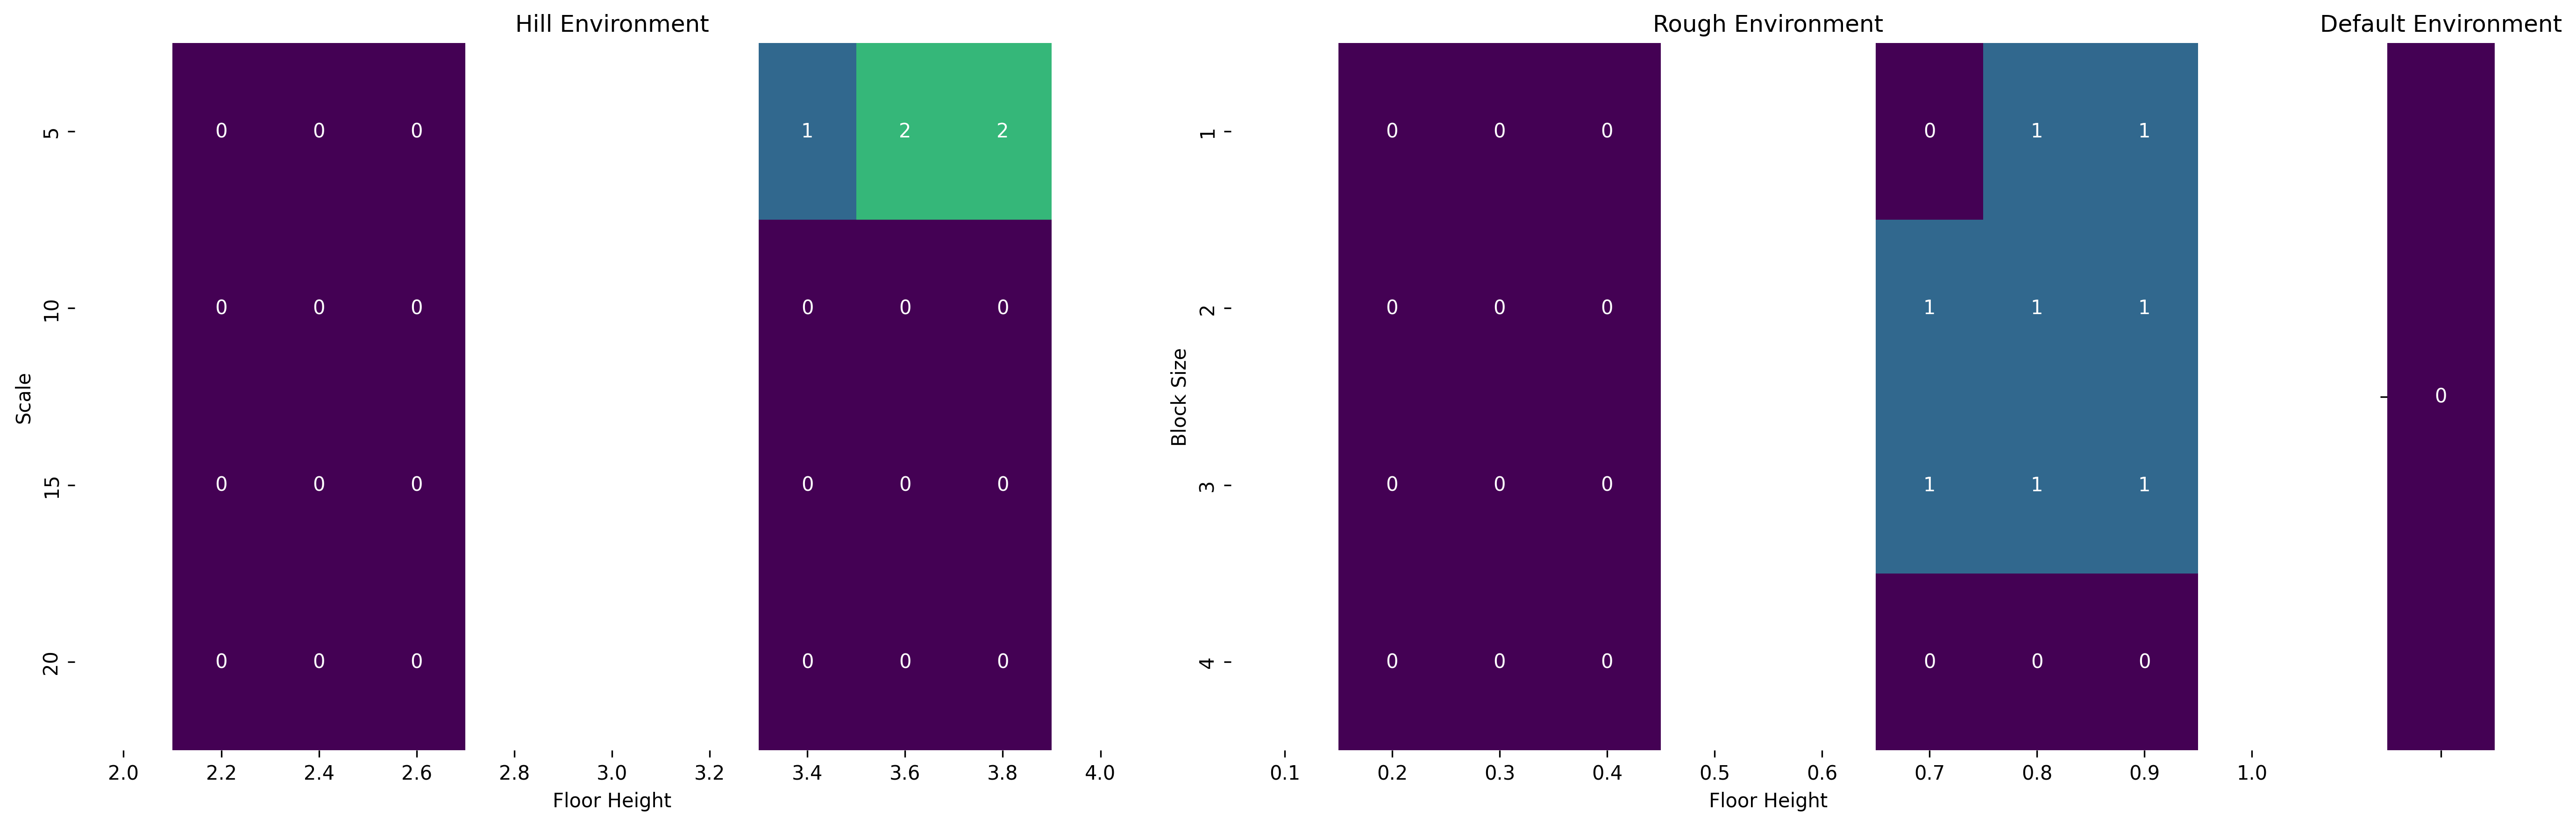
\includegraphics[width=\linewidth]{./resources/partition_5_2906_3/generalist_heatmap_partition.png}
                \caption{Figure showing to which partition the environment belongs to. In this experiment, three partitions where created.}
                \label{fig:heat_partition_number}
            \end{subfigure}

            \begin{subfigure}{\textwidth}
                \centering
                \begin{minipage}{0.19\textwidth}
                    \centering
                    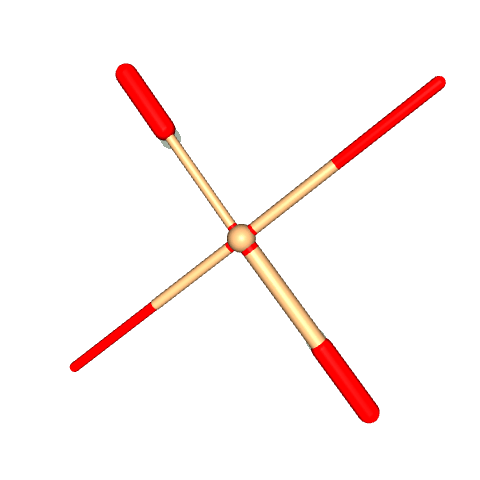
\includegraphics[width=\linewidth]{resources/partition_5_2906_3/ant_0.png}
                    \textbf{Partition 0}
                \end{minipage}
                \hfill
                \begin{minipage}{0.19\textwidth}
                    \centering
                    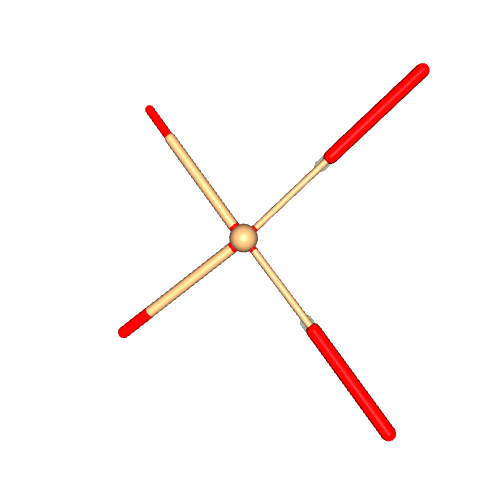
\includegraphics[width=\linewidth]{resources/partition_5_2906_3/ant_1.png}
                    \textbf{Partition 1}
                \end{minipage}
                \hfill
                \begin{minipage}{0.19\textwidth}
                    \centering
                    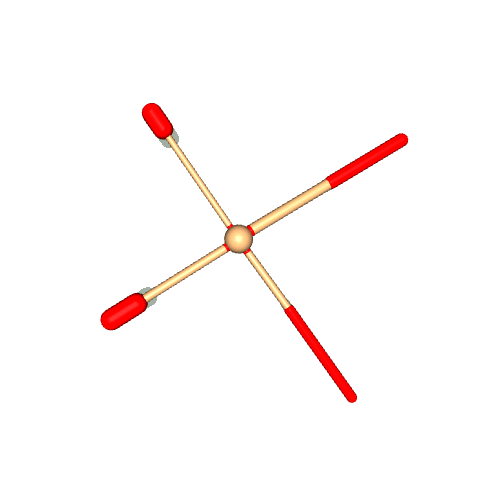
\includegraphics[width=\linewidth]{resources/partition_5_2906_3/ant_2.png}
                    \textbf{Partition 2}
                \end{minipage}
                \caption{Morphologies evolved for partitions of the environments}
                \label{fig:part_ant_images}
            \end{subfigure}

            \begin{subfigure}{\textwidth}
                \centering
                \begin{minipage}{0.32\textwidth}
                    \centering
                    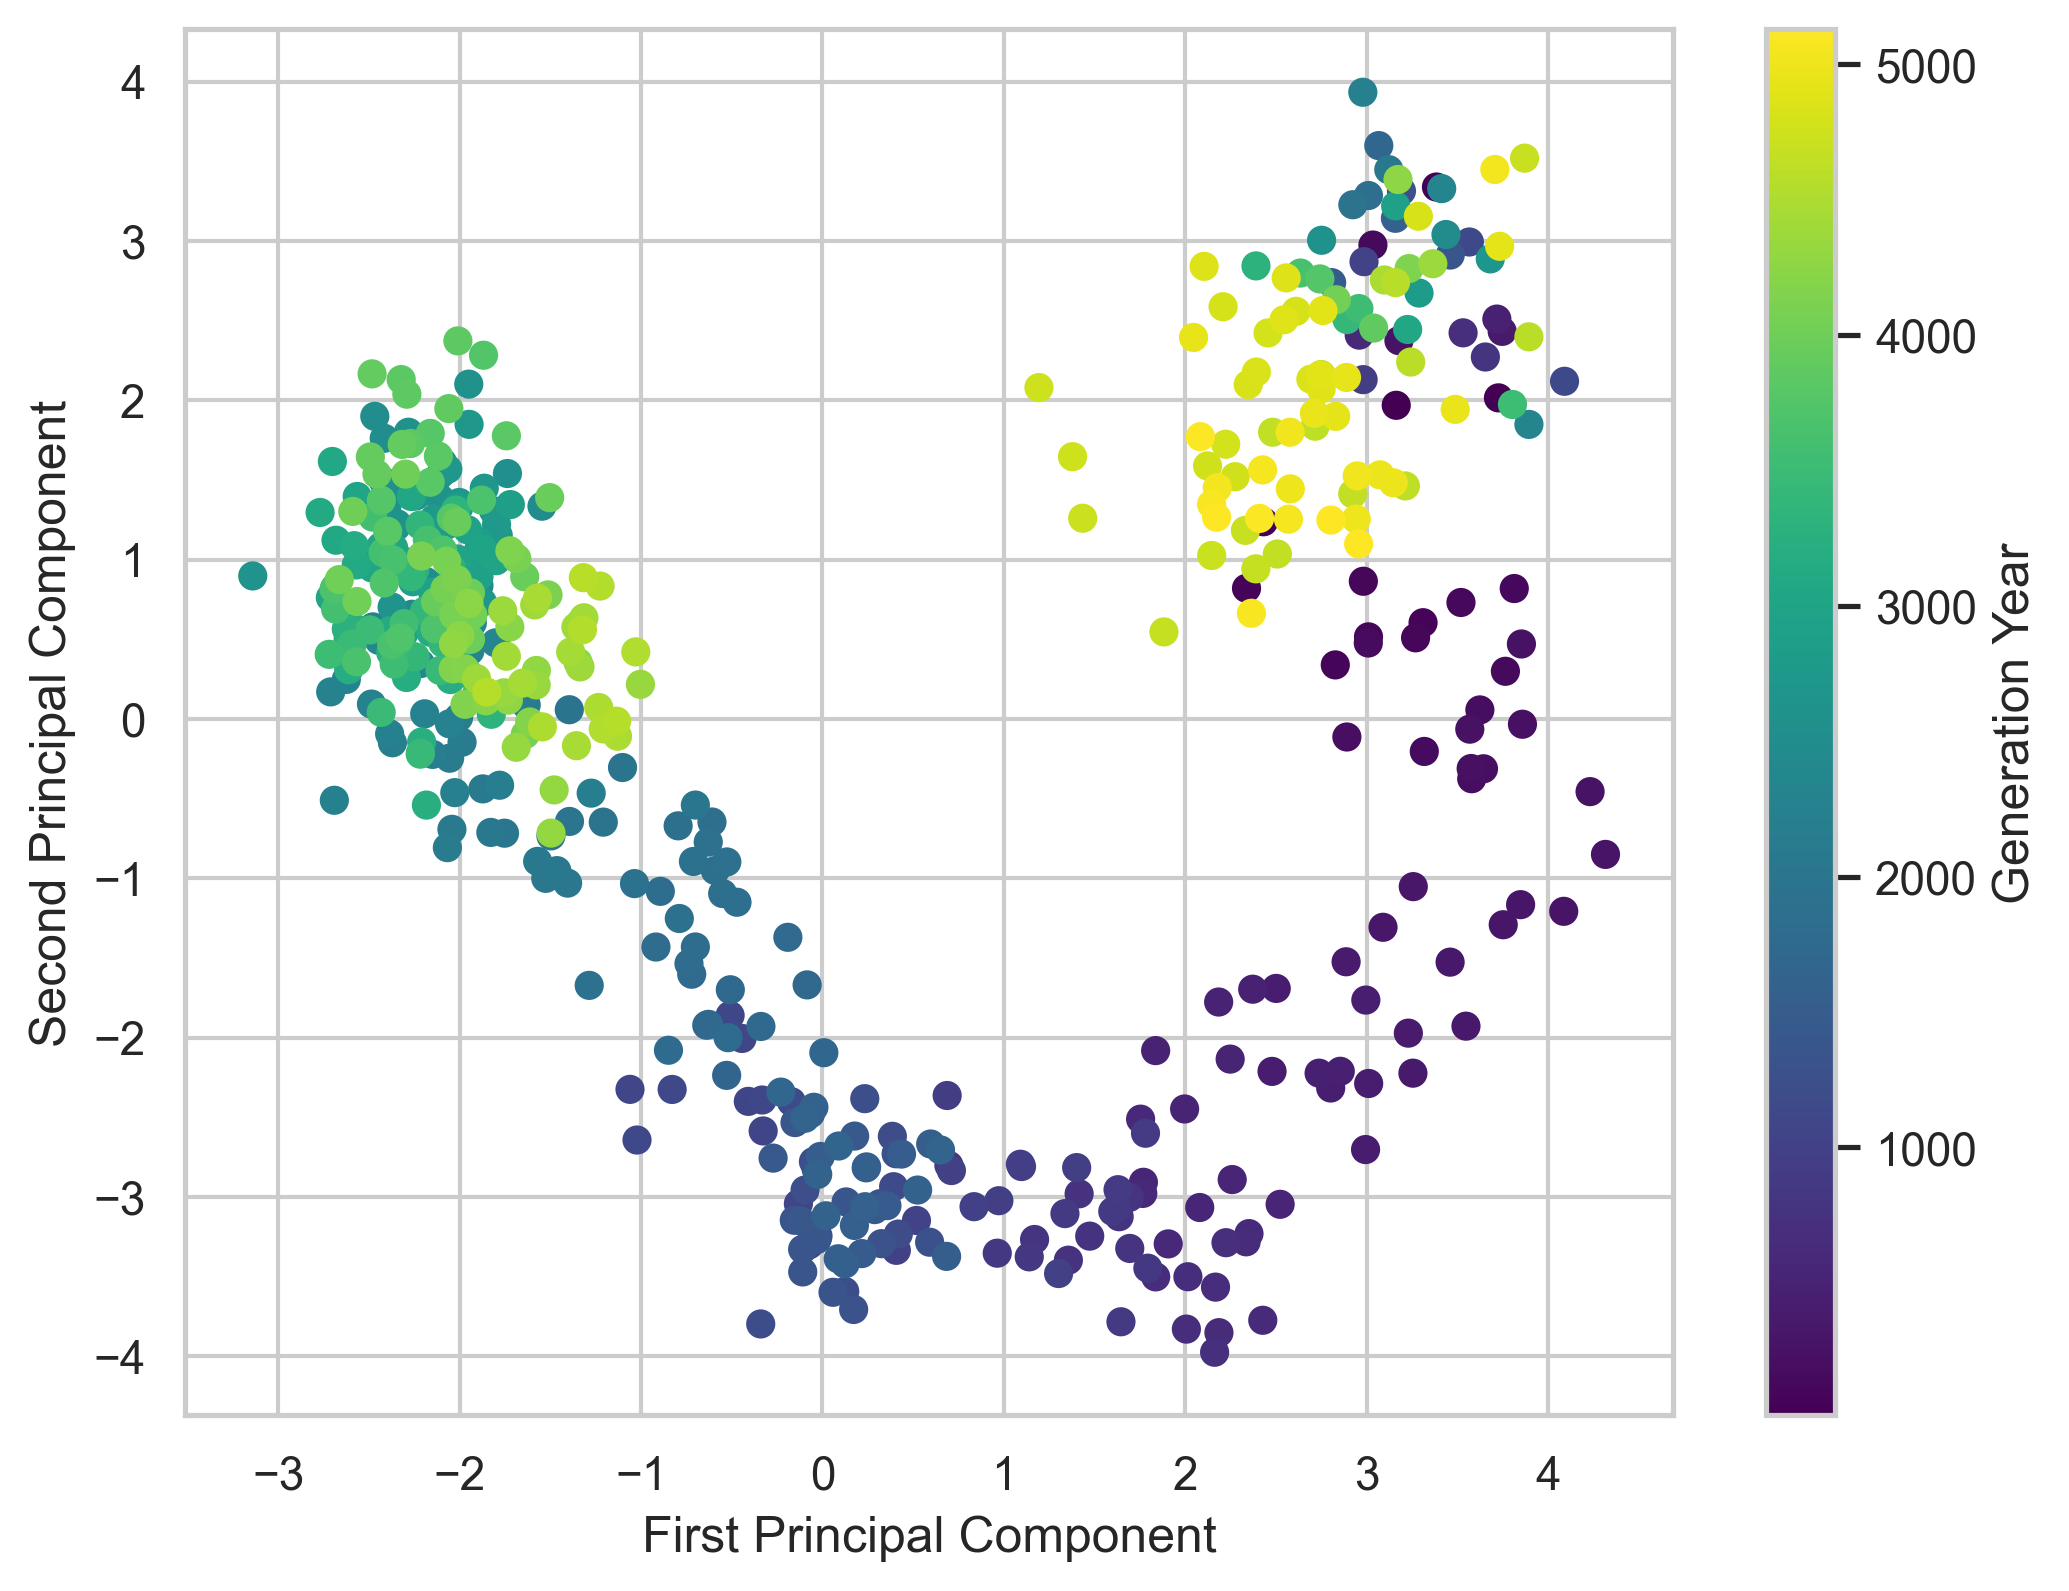
\includegraphics[width=\linewidth]{resources/partition_5_2906_3/partition_0/pca_scatterplot.png}
                    \textbf{Partition 0}
                \end{minipage}
                \hfill
                \begin{minipage}{0.32\textwidth}
                    \centering
                    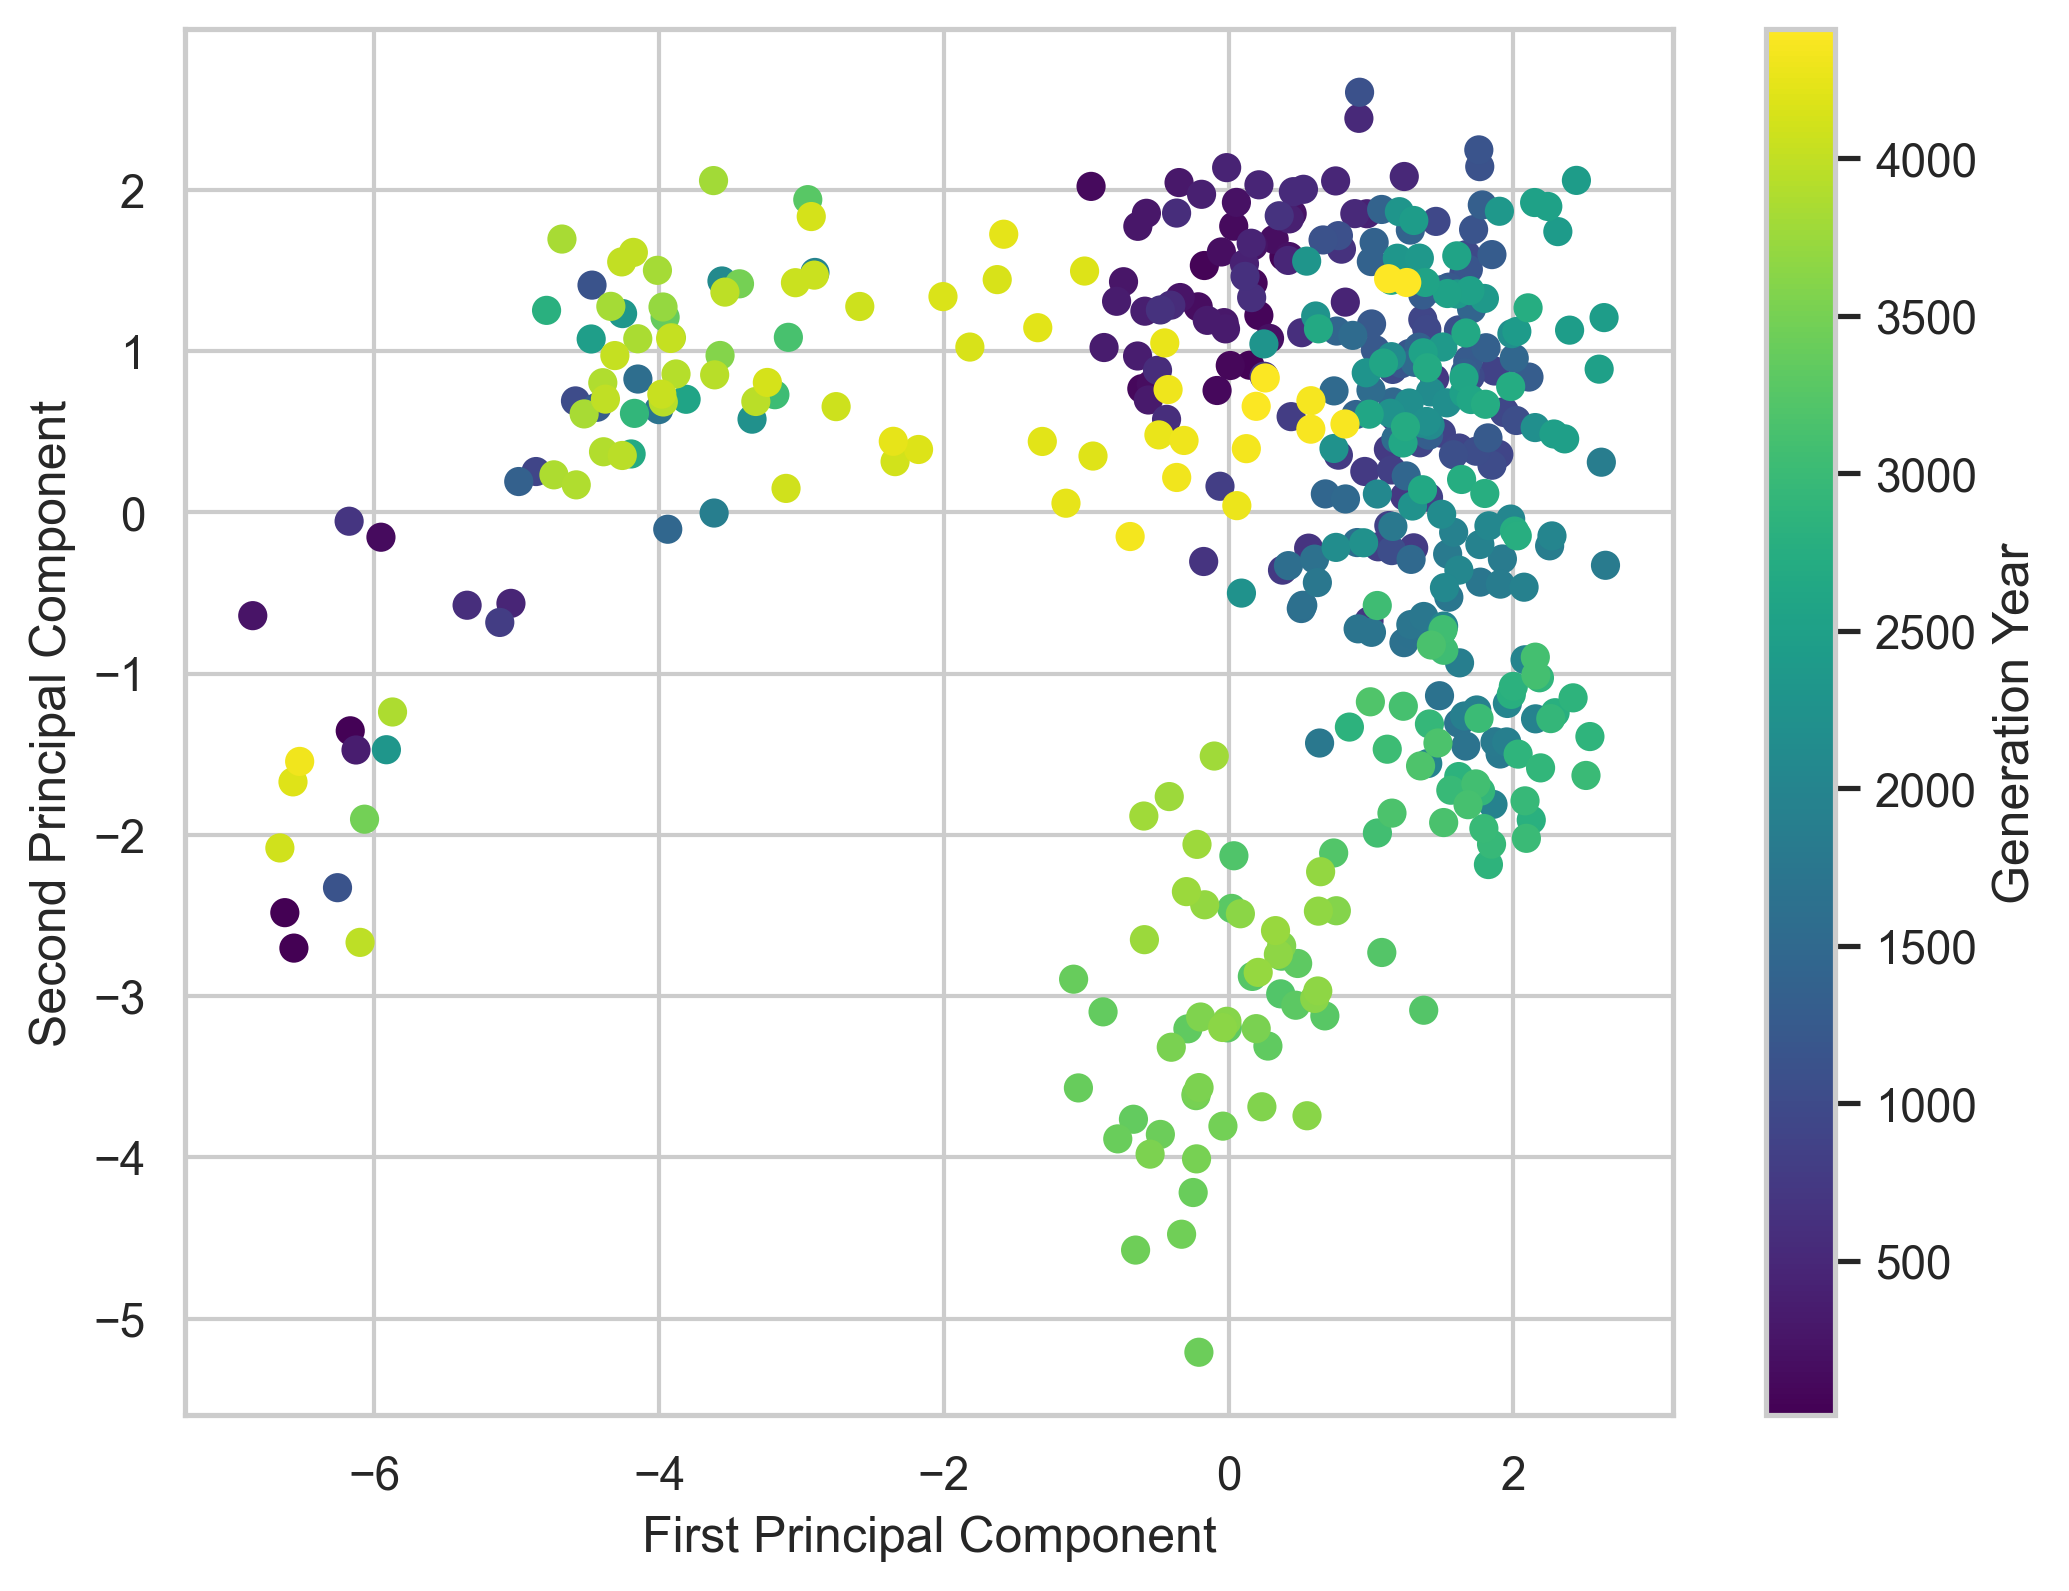
\includegraphics[width=\linewidth]{resources/partition_5_2906_3/partition_1/pca_scatterplot.png}
                    \textbf{Partition 1}
                \end{minipage}
                \hfill
                \begin{minipage}{0.32\textwidth}
                    \centering
                    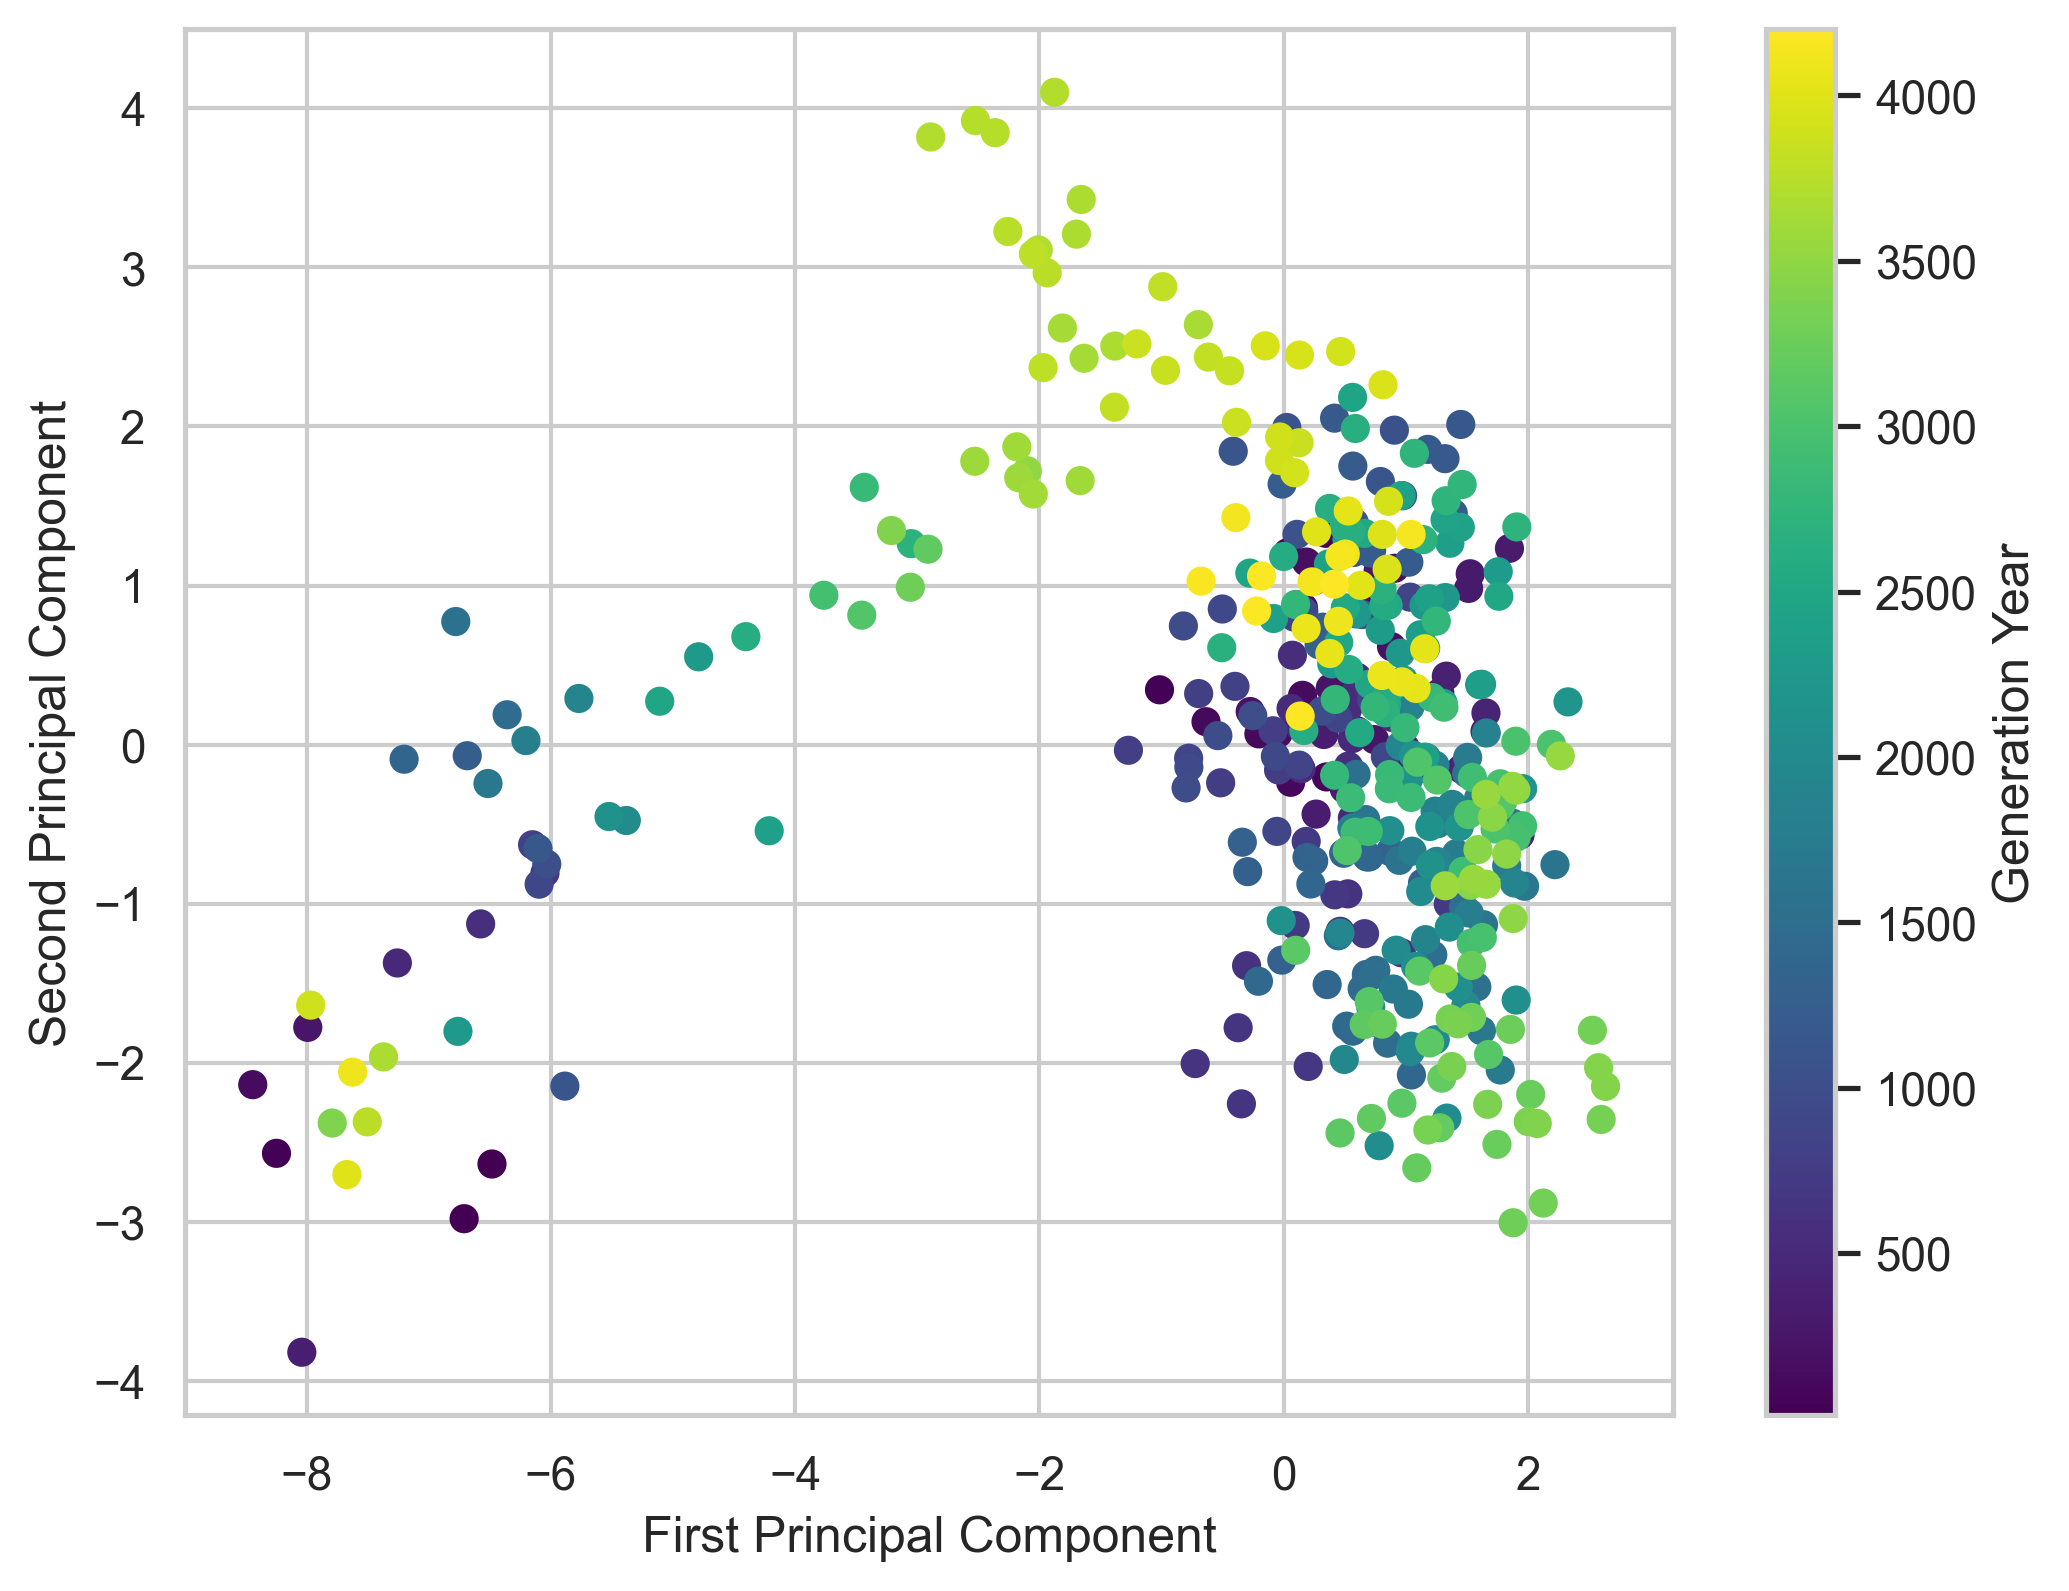
\includegraphics[width=\linewidth]{resources/partition_5_2906_3/partition_2/pca_scatterplot.png}
                    \textbf{Partition 2}
                \end{minipage}
                \caption{PCA scatterplots where the morphological parameters are reduced to 2 principal components.}
                \label{fig:pca_partition}
            \end{subfigure}

            \caption{Experiment 2 - Results of the second experiment where we evolve a set of generalist MC-pairs to handle a wide range of diverse environments.}
            \label{fig:experiment2}
        \end{figure*}

        Figure~\ref{fig:fit_heat_partitioned} shows the obtained fitness scores for each environment, represented in a heatmap for experiment 2. Similar to experiment 1, the hill environment shows high performance in the environments at the lower left, with relatively lower performance near the upper right. The fitness scores and their standard deviations for the training and testing sets are also similar. The training set has a mean fitness score of 3037.96 with a standard deviation of 1127.11, while the testing set has a mean fitness score of 3003.58 with a standard deviation of 1193.02. 

        For the rough terrain environment, the heatmap also shows high performance in the environments at the lower left and relatively lower performance near the upper right, and also in the lower right part, similar to experiment 1. The fitness scores on the training and testing sets are slightly different. The training set has a mean fitness score of 2812.58 with a standard deviation of 1016.59, and the testing set has a mean fitness score of 2679.42 with a standard deviation of 1215.64. 

        Overall, the set of MC-pairs do score a higher fitness on the rough terrain environment compared to experiment 1. This is evident when examining the partitions shown in figure~\ref{fig:heat_partition_number}. This figure presents the partitions to which each environment is assigned to. The blank white areas represent the testing environments that are not assigned to any partition. In this experiment, the environments in partition 1 and 2, that are being managed by another MC-pair, are of higher fitness scores, than in experiment one.

        The morphologies for each partition are visible in Figure~\ref{fig:part_ant_images}. The morphology in partition 0 is similar to the morphologies from experiment 1 in Figure~\ref{fig:gen_ant_images} with generalist scores 2412, 2784, and 3126. It also employs the same strategy to traverse the environment. This makes sense considering that experiment 1 is similar to the second experiment before partitioning. The morphology for partition 1 has two long front legs and two short back legs, where the back legs were used to propel itself, over the terrain. Lastly, the morphology in for partition 2 is comparatively smaller, featuring two back legs with thicker lower portions. It uses its front legs to latch onto a elevated terrain and subsequently try to climb it by then hooking its back legs to climb.

        The same PCA scatterplots where created for this experiment visible in Figure~\ref{fig:pca_partition}. These plots share many similarities with experiment 1 and do not reveal anything more compared to the plots from experiment 1.

    \subsection{Experiment 3: Specialist for each environment}
        \begin{figure*}[!ht]
            \centering
            \begin{subfigure}{\textwidth}
                \centering
                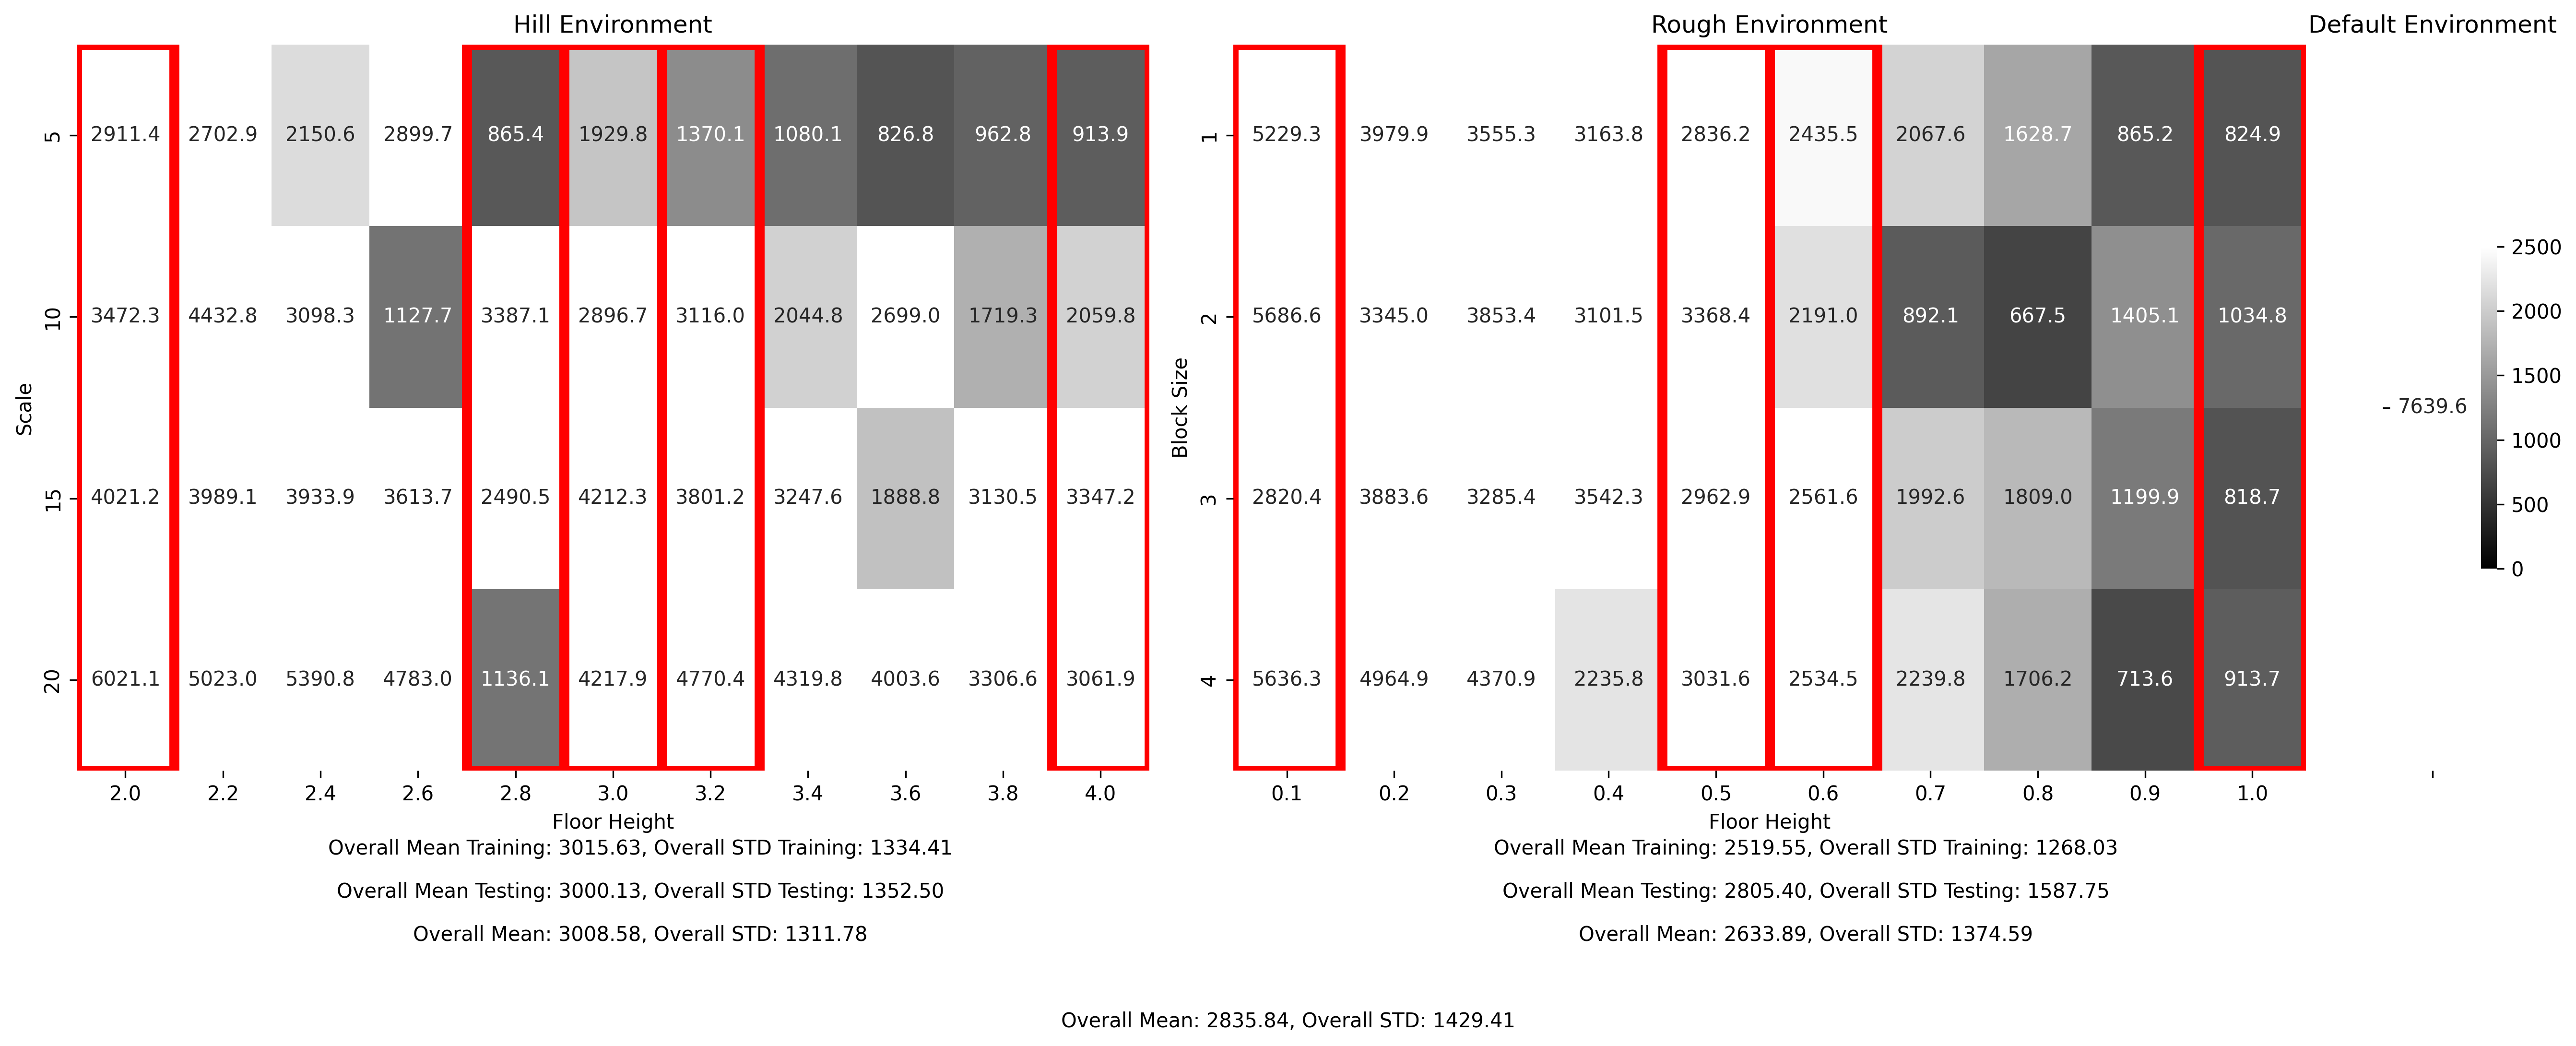
\includegraphics[width=\linewidth]{./resources/specialist_1_2835/fitness_heatmap.png}
                \caption{Fitness heatmap of a specialist MC-pair for each environment.}
                \label{fig:fit_heat_spec}
            \end{subfigure}

            \begin{subfigure}{\textwidth}
                \centering
                \begin{minipage}{0.19\textwidth}
                    \centering
                    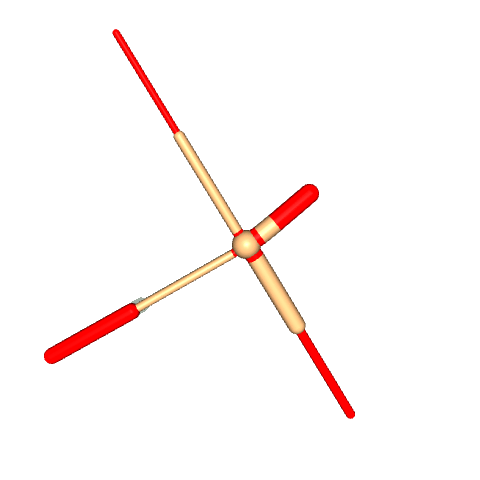
\includegraphics[width=\linewidth]{resources/specialist_1_2835/rough_4_0.4.png}
                    \textbf{Rough terrain Block size: 4 Floor height: 0.4}
                \end{minipage}
                \hfill
                \begin{minipage}{0.19\textwidth}
                    \centering
                    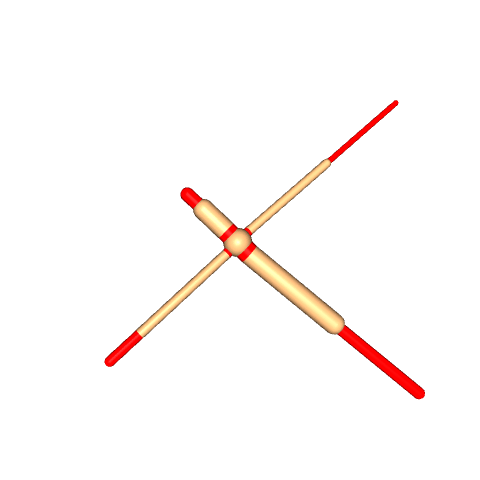
\includegraphics[width=\linewidth]{resources/specialist_1_2835/default.png}
                    \textbf{Default terrain}
                \end{minipage}
                \hfill
                \begin{minipage}{0.19\textwidth}
                    \centering
                    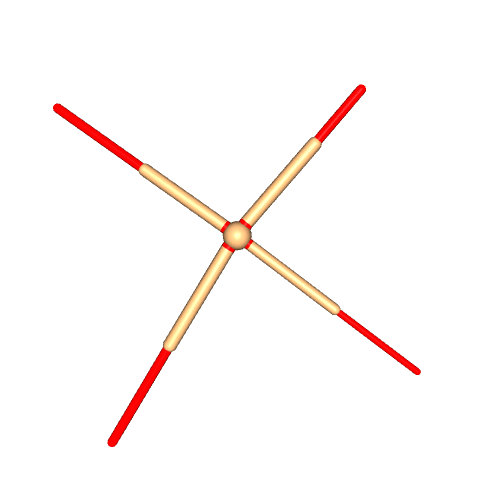
\includegraphics[width=\linewidth]{resources/specialist_1_2835/hills_20_2.0.png}
                    \textbf{Hills terrain Scale: 20 \newline Floor heigth: 2.0}
                \end{minipage}
                \caption{Specialist morphologies each evolved for one environment. The specific environment the morphology was evolved in is shown below the image.}
                \label{fig:spec_ant_images}
            \end{subfigure}

            \caption{Experiment 3 - Results of the third experiment where we evolve a specialist MC-pair for each individual environment.}
            \label{fig:experiment3}
        \end{figure*}

        Figure~\ref{fig:fit_heat_spec} shows the fitness scores obtained for each environment in experiment 3, represented as a heatmap. Unlike the results seen in experiment 1 and 2, this heatmap has a less distinct gradient. Fitness scores for some environments are lower than in the previous experiments, while others are higher. The overall mean fitness score across all environments is 2835.84 with a standard deviation of 1429.41. Although the is comparable to the previous experiments, the standard deviation is significantly greater, indicating more variability in the fitness scores. Notably, in the more complex environment, it was more challenging to evolve a performant specialist MC-pair, whilst the generalist scored higher. 
        
        Some interesting morphologies for some environments with unique strategies are showcased in Figure~\ref{fig:spec_ant_images}. The first morphology was evolved in the rough terrain environment with block size 4 and floor height 0.4. This terrain has larger size blocks elevated, requiring the ant's torso to be higher than the blocks in order to move forward. The long and thin leg was primarily used to lift the ant slightly into the air, while the other three legs were used to lunge itself forward. The second morphology was evolved in the default terrain environment. This terrain is completely flat, with no obstacles that could hinder the ant's forward motion. The two long and thin sidelegs are mainly responsible for the forward motion, while the longer front leg and very short back leg are mainly responsible for its balance. The front leg remains mostly still, only correcting the ant if it tips too far forward. The back leg does not touch the ground, but constantly makes a waggling movement. The third morphology was evolved in the hills terrain environment with scale 20 and floor height 2.0. The hills in this terrain are more stretched out and not as high, resembling a bit more to a flat environment. The ant looks almost symmetrical, with one leg bit longer then the rest. Each leg equally contributes to the forward movement, making it resemble an actual ants movement more. 



